\documentclass{article}
\usepackage[utf8]{inputenc}
\usepackage[english]{babel}

%Used to write discontinuous functions 
\usepackage{amsmath}
% used to write norm
\usepackage{mathtools,xparse}
\DeclarePairedDelimiter{\norm}{\lVert}{\rVert}

\usepackage[lmargin=25mm,rmargin=25mm,tmargin=27mm,bmargin=30mm]{geometry}

%Enable use of pgf figures
\usepackage{pgfplots} 

% err math function
\DeclareMathOperator\err{err}

%citing: write all articles in the .bib file. Only the ones that are cited in the project will appear
% in the bibliography
\usepackage{biblatex}
\addbibresource{references.bib}

%getting bold symbols in math mode
\usepackage{bm}

%getting unumbered subfigures
\usepackage{caption}

\title{Machine learning for condition monitoring of hydro electric powerplants}
\author{Asgeir Øen Åsnes }
\date{\today}

%Remove intendation at newline
\usepackage[parfill]{parskip}
%Centering pgf images
\usepackage{tikz}
\usepackage{pgf}


\begin{document}
\pagenumbering{gobble}
% !TEX encoding = UTF-8 Unicode
%!TEX root = thesis.tex
% !TEX spellcheck = en-US

%This is the Titlepage
%%=========================================

\begin{flushleft}
\begin{figure}[t]

\includegraphics[height=3cm]{figures/ntnulogo.jpg}
\end{figure}


\LARGE{Machine Learning for Condition Monitoring}
\newline
\LARGE{in Hydro Electric Powerplants}

%\maketitle{}
\vspace{3cm}
\Large{Asgeir Øen Åsnes}\\


\vspace{6cm}




\normalsize{Project Thesis, Cybernetics and Robotics\\
\noindent Supervisor 1: Lars Imsland (ITK, NTNU)\\
\noindent Supervisor 2: Anders Willersrud (Hymatek Controls)}
\vfill

\normalsize{Department of Engineering Cybernetics\\
Norwegian University of Science and Technology\\}
\end{flushleft}




\newpage
\pagenumbering{roman}
\section*{Preface}
    This project thesis is written as a part of my Master's degree in Cybernetics and Robotics at NTNU Trondheim. The work is done during the fall of 2017. This project looks into condition monitoring of a mechanical component in a hydro electric powerplant. Machine learning techniques are used to try to classify the condition of the component. I chose this project because I wanted to learn more about machine learning, and to see how it can be utilized on condition monitoring in the industry. This also meant that I could benefit from my practical experience with maintenance in the industry, from working as a ship electrician offshore. The project is a collaboration between NTNU and Hymatek Controls.  

    
    \begin{center}
    Trondheim, \today \\
    \vspace{1.5cm}
    Asgeir Øen Åsnes
    \end{center}
\clearpage

\section*{Abstract}
    Databased methods are used to try to classify the condition of the guide vanes in a Francis turbine in a hydro electric power plant. The data is taken from a large hydro electric power plant in Norway. The plant has four identical generator sets, with different maintenance schedules. They are therefore used as examples on how a plant changes over time. The analysis is performed using the following machine learning techniques, support vector machines, logistic regression and neural networks. There are two different datasets available for all the four turbines. A servo indication dataset, which today is used to manually estimate the condition of the guide vane system, and a dataset from commissioning. The performance of the different algorithms on the two different datasets are analyzed, to see which shows most promise. It is attempted to find out if data from commissioning holds the same information as a servo indication.  
    
    
    The results shows that the servo indication data set is the easiest to extract information from. All the different algorithms were able to detect change in the condition of the turbines. The neural network and one class support vector machine gave the best results. The neural network had a prediction accuracy above $90\%$.  
    
    For the commissioning data, only one algorithm, the one class SVM gave useful results. The other algorithms were not able to handle the amount of non informative data included in the commissioning dataset. The other classifiers run into problems with the distribution of the data samples.  The one class support vector machine is however capable of producing almost the same results for the commissioning data, as it was for the servo indication. 


    The oneclass SVM could give useful information about a turbine based on the results from the commissioning data.  However data from normal operation over a longer period might not be comparable to the commissioning data. But, one can argue that if one can figure out how to estimate the condition of the guide vanes from a classifier such as the one class SVM, it might not be necessary to perform a servo indication. The commissioning data seems to hold much of the same information.
    
    
\clearpage    

\section*{Contents}
\makeatletter
\@starttoc{toc}
\makeatother
\newpage


% \listoffigures
 
% \listoftables

%Main matter 
\pagenumbering{arabic}


\section{Introduction}
    \subsection{Background}
        The Norwegian electrical grid is almost exclusively provided by power generated by hydro electric power plants \cite{Energi212014}. Many of the biggest power plants have been producing power for over five decades \cite{vannkraft}, and many of them are in need of upgrades \cite{tu}. Hydro electric power plants are now and then stopped for maintenance. This is in some cases of course unavoidable, since all equipment has a certain life span, and hence needs replacement, but in many cases components are overhauled and changed without showing signs of wear and or damage. 
        
        
        
        
    \subsection{Motivation}
    
        Two important factors in a hydro electric power-plant follow. Firstly, it is important that all the rainwater collected is used to produce power. This means that having reservoirs so full that they flood over is like throwing money into the river. Secondly as with all power plants, you want to produce most of your power when the prices are as high as possible. This can be solved by keeping the plants power production, and hence water usage at optimal levels at all time. This again means that you can optimize your production, as long as your plant is operable. Another important factor is the fact that hydro electric power is a clean power source. In a world that desperately needs clean power, every little improvement is welcome addition. 
        
        
    \subsection{Problem definition}    
        In hydro electric power plants today, there is little to no condition estimations. Maintenance is scheduled based on running hours, planned maintenance or break downs. This project looks into condition monitoring for a very specific part of a hydro electric power plant, the dead band of the guide vanes for a Francis turbine. The guide vanes are what controls  how much water is led onto the turbine at any given time. These guide vanes are controlled by one or two hydraulic motors, through a series of mechanical components. Figure \ref{fig:servo_plant} shows such a servo motor controlling the guide vanes. As a turbine system ages, the dead band of the guide vanes increase. The dead band explains how much differential force is need to change the direction of motion of the guide vanes, from opening to closing or closing to opening. This can be compared to the dead band found in valves \cite{Choudhury2005}. The dead band is connected to the friction coefficient of the guide vanes. As the guide vanes are worn down, the friction increases, and so does the dead band.  
        
        % \begin{figure}
        %     \begin{minipage}[b]{0.5\linewidth}
        %         \centering
        %         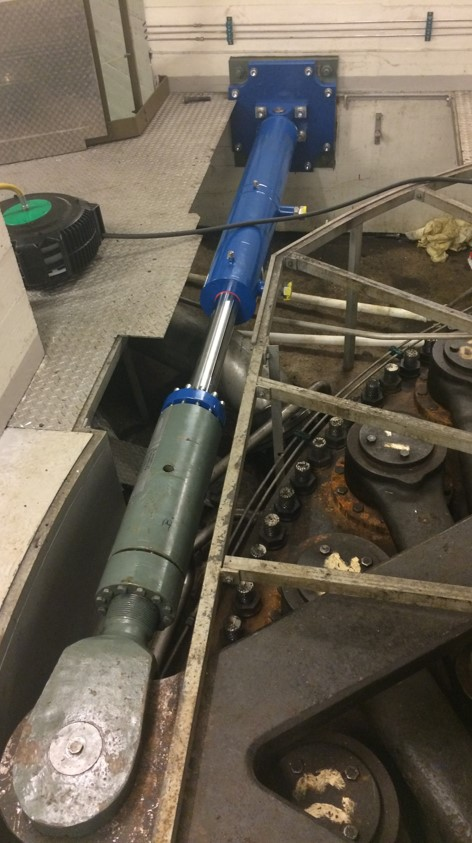
\includegraphics[scale = 0.5]{figures/introduction/servo1.jpg}
        %         \caption{Servo motor for either closing or opening at an actual plant. It is connected to a ring which controls the opening of the guide vanes. Courtesy of Hymatek Controls.}
        %         \label{fig:servo_plant}
        %     \end{minipage}
        %     \hfill
        %     \begin{minipage}[b]{0.5\linewidth}
        %         \centering
        %         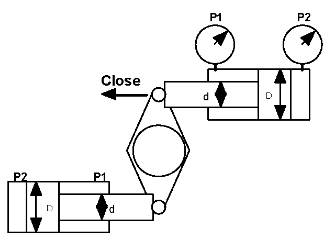
\includegraphics[scale = 0.5]{figures/introduction/servo.png}
        %         \caption{Schematic showing the how the opening and closing servos act upon the system.}
        %         \label{fig:servo_schematic}
        %     \end{minipage}
        % \end{figure}
    
        \begin{figure}
            \centering    
            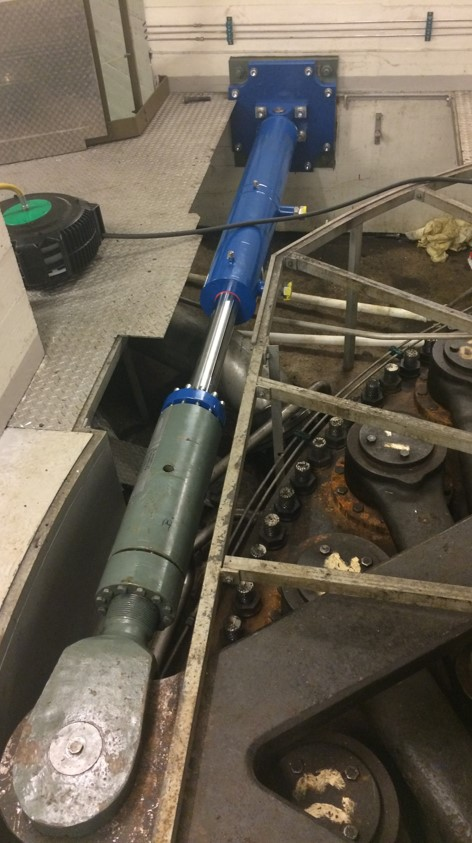
\includegraphics[scale = 0.5]{figures/introduction/servo1.jpg}
            \caption{Servo motor for either closing or opening at an actual plant. It is connected to a ring which controls the opening of the guide vanes. Courtesy of Hymatek Controls.}
            \label{fig:servo_plant}
        \end{figure}
        When the friction becomes too large, the hydraulic system will not be able to control the system as wanted. Today the condition of the guide vanes and its mechanical components are found by disconnecting the generator from the grid, and performing a servo indication. By disconnecting the generator from the grid the water flow over the turbine can be manipulated without having to worry about output voltage and frequency. It is crucial that the procedure is performed so slowly that the footprint of the water power is negligible. 
        
        When a generator is delivering power to the grid, wast amounts of water are flowing through the system at any given time. The guide vanes are adjusted with respect to the power the generator is delivering to the grid. Changes in the restriction of water flow (change of guide vane position) can generate disturbances and overshoot in the system. This can be spotted as noise in the measured process signals. When a servo indication is performed, the rate of change of water restriction (changing of the guide vanes position) is so slow that the effects from the water are minimized. This gives much cleaner process signals, that are easier to analyze, because they mostly consist of data relevant to the dead band estimation.
        
        However if it could be possible to create an estimate of the dead band and hence the friction coefficient during normal operation, this would be very beneficial. Firstly this will reduce costs. Today the analysis are outsourced to consultants, and they need to mount new equipment to take the necessary measurements. This again leads to increased plant activity. Secondly, downtime due to an hour based maintenance schedule, can be reduced. Finally, it introduces a constant estimate of the condition of the plant, something that is not available today. This is however not a straight forward thing to solve. To begin, creating a classifier which enables detection of changes in the condition of the guide vanes is a natural first step. This is the focus of the project. The guide vane friction issue is similar to problems found in valves. According to \cite{Dozat} there is a clear need for methods to detect and quantify the stiction in valves. Hence, if one can find a solution to estimating the condition of the guide vanes, this might be applicable to the process industry as well. 
        
        
    \subsection{The techniques used}    
        Building a model for the dead band of the guide vanes is complex. There can be complex hysteresis effects, and the shape of the curve can be very nonlinear. An example of the deadband of a guide vane system is shown in Figure \ref{fig:deadband}. There are even worse cases where the "banana" shape becomes even steeper and narrower at the ends. These nonlinearities makes it hard to create a general model. Each turbine has its own maintenance schedule, and they might not have the same mechanical components. This means that a model that works great for one system, might not be valid at all for another. Therefore, it has been chosen to focus on databased methods, to try to create a classifier for the condition of the guide vanes. These can be trained on measurements taken from each individual turbine, reducing the time and cost compared to creating a mathematical model for each. 
        
        \begin{figure}
            \centering
            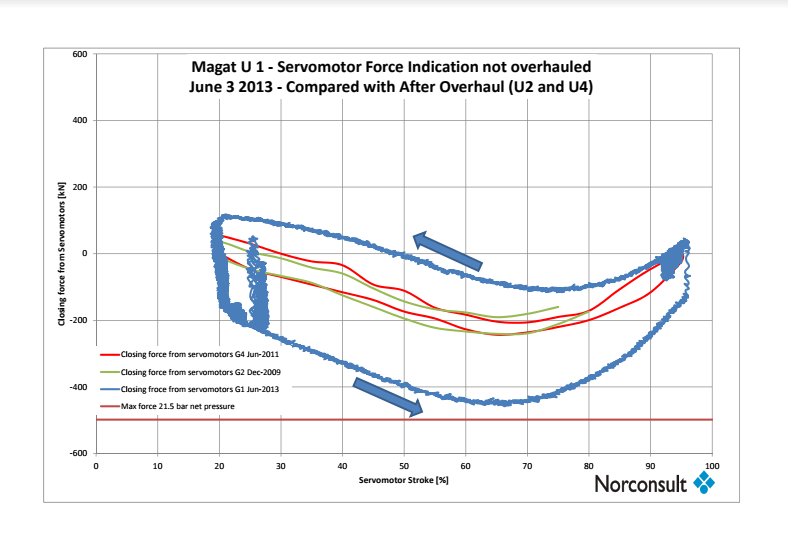
\includegraphics[width=0.8\textwidth]{figures/introduction/deadband.png}
            \caption{Deadband of servoindication, courtesy of Norconsult}
            \label{fig:deadband}
        \end{figure}

        As for the data based methods, three separate methods have been chosen. Most importantly because they span machine learning from simple to advanced. If the problem can be solved using a simple method, there is no need to use a more complex one. Also, the simpler machine learning methods are the ones easiest to interpret in how they separate the data. For this project, logistic regression, support vector machines and neural networks are the methods chosen. Each of them will be tested and compared to one another. 
        
    \subsection{Case studies}   
        As mentioned in the motivation section, this project looks into condition monitoring of the guide vanes found in a Francis generator. The data available for analysis comes from four similar generator sets, with different running hours since last overhaul. This means that the four different data sets, can be viewed as coming from the same generator over many years. Hence these four cases, can be used to create classifiers that can classify the condition of the generator into four different classes, from good to bad. The datasets consist of a series of time-series data samples stored in a series of .csv files. These time-series are taken during commissioning and servo indication. %Figure \ref{fig:data} shows the different variables found in the data set.
        
        Today the servo indications are manually analyzed by engineers. Hence enabling automatic classification based on a servo indication measurement will be a step forward. This is the first case looked into. One servo indication dataset is available for each of the four generators. The first task is then to create a classifier that based on the servo indications are able classify the condition of the guide vanes into four different categories. Notice that here only classification is looked into, it is not made an attempt to estimate the actual level of friction in the guide vanes.
        
        The second task, is trying to recreate similar classifiers, based on measurements taken during commissioning of the same generators. These measurements include disturbances and might be more difficult to analyze than the pure servo indication data. If it could be shown possible to find dead band information from these noisy data measurements, this is a step towards enabling real time assessment of the condition of the guide vanes, and remove the need for taking servo indications.

        % Insert image of the four different cases. 
        
        % \begin{figure}
        %     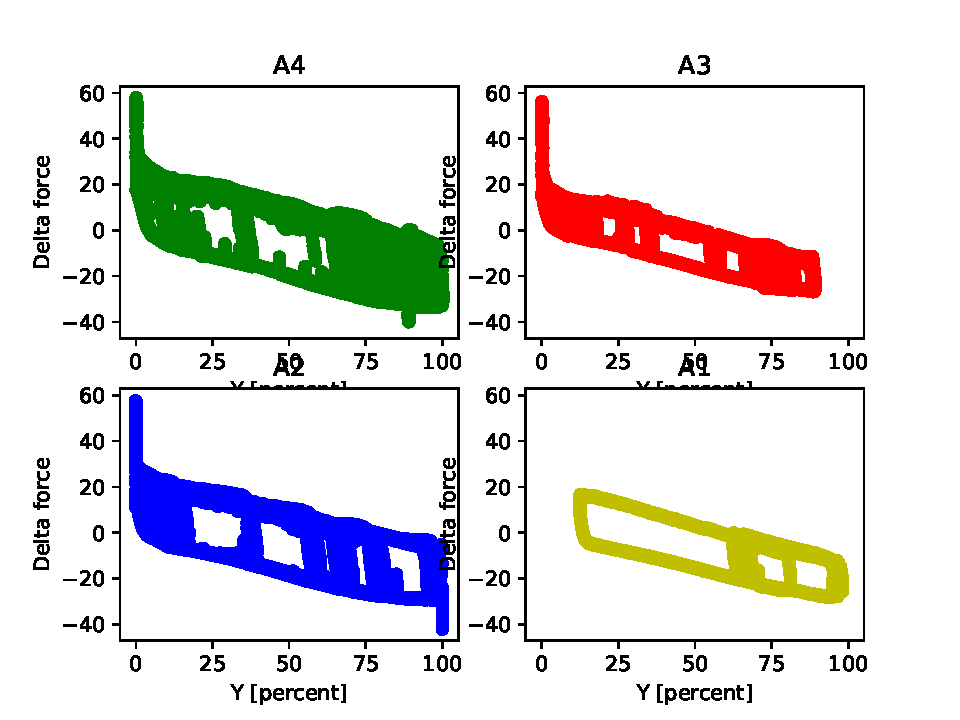
\includegraphics[width=\textwidth]{figures/introduction/ServoIndicationsub.pdf}
        %     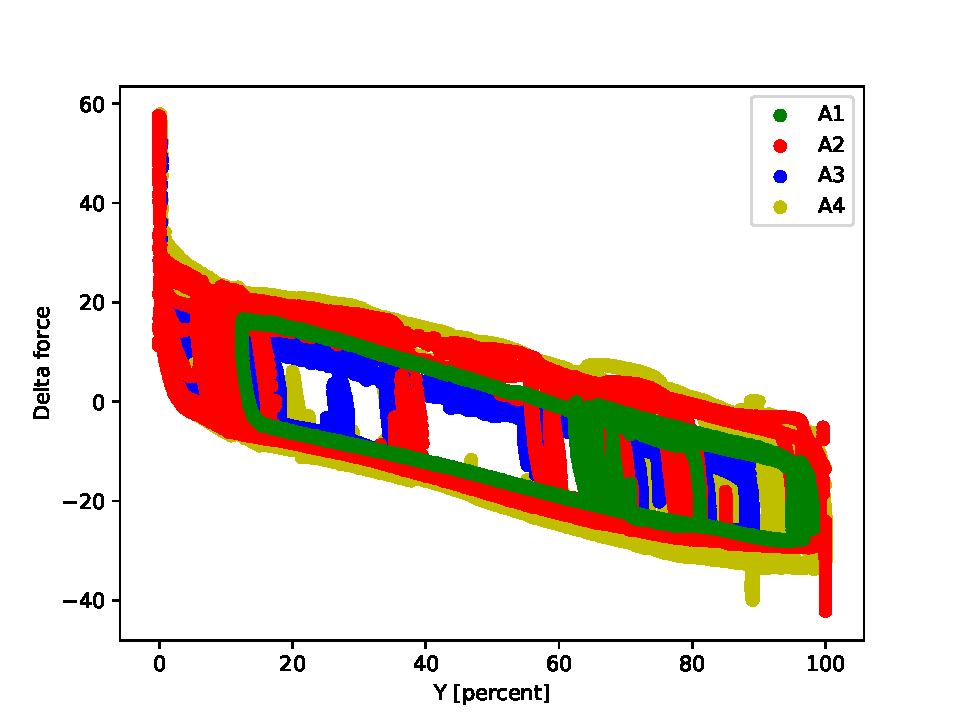
\includegraphics[width=\textwidth]{figures/introduction/ServoIndication.pdf}
        % \end{figure}
        
        
        
        
        
    % \subsection{Literary analysis}
    
    %     overordna, condition monitoring
    %     hydropower
    %     cm on hydraulics?
    %     State of the art of condition monitoring of hydraulics at the moment? 
        
        


\section{Machine learning}
    
    This section serves as an introduction to the machine learning algorithms worked with in this project. Logistic regression, support vector machines and neural networks are the algorithms used. They are presented to give an intuitive understanding of how they work. What is presented in this section is mostly based on \cite{Hastie}. In addition a lot of the intuitive understanding comes from Andrew Ng's online courses, \cite{machinlearning} and \cite{deepLearning}.
    
    The methods used in this project have been chosen because they span the machine learning universe from simple to advanced. Firstly, this is done to ensure that one does not use unnecessary complicated methods. If simpler methods are good enough, they might be easier to interpret than the more complex ones. Secondly, more complicated methods will most likely give longer training and run-time. Two Python libraries are used for the analysis. Scikit-learn \cite{scikit-learn}, \cite{scikit-web} for logistic regression and support vector machines, and Keras \cite{chollet2015keras} for neural networks. There are a number of different libraries available, but these are chosen due to their ease of use, and the fact that Keras has an API that allows it to be used through Scikit-learn. This means that a lot of code can be reused when using the two libraries. 
        
    
    \subsection{Terminology}
        To simplify the further reading, some of the terminology used further is explained here. 
        
        \begin{itemize}
            \item ML, short of machine learning
            \item A variable is in ML referred to as a feature
            \item One data sample is also known as a feature vector, av vector holding the value of each of the features for this variable
            \item A class, is one of the different groups a feature vector can belong to.
            \item In classification you have a limited number of possible classes a feature vector can belong to. If you don't have a limited number of classes, regression  can be used to estimate the value.  
            \item For classification, a label tells you which class a feature vector belongs to.
            \item NN, short for neural network
            \item SVM, short for support vector machine
            \item LR, short for logistic regression
            \item Objective/scoring function, function used by the algorithm to optimize the results. 
        \end{itemize}
    
    \subsection{Supervised vs unsupervised algorithms}
        There are two main classes of machine learning algorithms, supervised and unsupervised. In supervised algorithms, you have labeled data. This means that you have data from the different types of scenarios you want to analyze. Say you want to build a machine learning algorithm that estimates the value of your used car. Then you need to collect information of already sold cars, the price they were sold for and a set of car features. Examples of useful features would be engine size, mileage, color, seats, drive type etc. Now you have a labeled dataset where each car with its features have a labeled price. You can then use supervised learning to train a classifier based on the data set, which you then can use to estimate the price of your car. In unsupervised learning, the price of the sold cars are unknown. What can be done here, is to analyze the data and look for unknown common structures. It is basically a grouping algorithm, that groups similar feature vectors together, which then later can be used to classify new feature vectors. 
        
        Supervised algorithms can again be split into two different sections. Regression or classification. In regression you have a continuous output range, as with the car example above. Then you want your algorithm to give you an estimate of the car price with an exact value. In classification however, you have a set of classes you want to classify all your data with. One might not need an accurate prediction of the price of a car, instead an estimated price range might be good enough.
        
    
    \subsection{The different algorithms}
        
            
            Note that the mathematical explanation of the algorithms are general approaches to explain how they work, the algorithms used does not necessarily use the exact same equations, but the general idea is similar. 
        
        \subsubsection{Linear regression}
            Linear regression serves as a good introduction to how machine learning works. It is also the basis for Logistic regression which is used in this analysis. Linear regression finds the best linear solution to your estimation problem. Based on you input features and labels for the data points, a linear function is fitted to the data. This is done by minimizing 
            \begin{align}
                J(\bm\theta) = \frac{1}{2m} \sum_{i=1}^{m}(h_\theta(\bm x^i) - y^i)^2.
                \label{linreg:cost}
            \end{align}
            
            You want the prediction 
            \begin{align}
                h_{\theta}(\bm x) = \theta_0 + \theta_{1}x_1 + \theta_{2}x_2 + ...+ \theta_{n}x_n,
                \label{linreg:h}
            \end{align}
            
            to be as close to $y^i$(the label) as possible. To continue the example with car prices from the section above, $h_\theta(x^i)$ will then be the linear function that estimates a cars price, based on $\bm x$. $y$ will be the actual price the cars were sold for. Equation \ref{linreg:h} shows the prediction function $h_\theta(x)$. As can be seen each feature in the feature vector, is multiplied with one unique coefficient. Since the function that best predicts the outcome is unknown, these coefficients can be randomly initialized. Chapter 3.2 in \cite{Hastie} explains in detail about how to sample the coefficients.  
            
            The optimal coefficients for $h_\theta(x^i)$ is found in an iterative approach. The most straight forward approach is gradient descent 
            
            \begin{align}
                \theta_i = \theta_i - \alpha \frac{d}{d\theta_i}J(\bm x).
                \label{linreg:gd}
            \end{align}
            
            
            There are many different options for the solver in machine learning, gradient descent is the simplest one of them. Better performance can be found using more advanced solvers. However this is not a part of the cases looked into here, so gradient descent is used for explanation, and the different algorithms are run with the solver that yields best performance. Equation \ref{linreg:gd} shows the update steps using gradient(steepest) descent. The partial derivative of $J(\theta)$ is found for each of the $\theta_i$, this explains how much $J(\theta)$ changes with respect to $\theta_i$. The $\alpha$ is a tunable parameter known as the learning rate. It should lie somewhere between zero and one. The larger you make $\alpha$, the faster your algorithm will move through the solution space. By first intuition one should think that the bigger $\alpha$ the better, but it can be shown that a too large $\alpha$ can lead to divergence. $\alpha$ should be as big as possible but still small enough to avoid this issue. A small $\alpha$ will change the coefficients very little for each iteration, making the search exhaustive, and will in worst case run forever. This is an example of hyperparameterization which is discussed in more detail in a later section. 
            
            Despite the name, linear regression can also be used to find nonlinear decision functions. This is done by adding nonlinear features to the feature vector based on the original features, one example is polynomial extension. Say the original feature set is, $x_1$ and $x_2$. By creating new polynomial features to the second degree, the augmented feature vector will become $[x_1, x_2, x_1^2, x_2x_1, x_2^2 ]$. This now enables the linear regression algorithm to find nonlinear decision functions. In theory this enables linear regression to find any decision function, however this needs the polynomial to grow very large. This again leads to an enormous growth in features. The speed of the algorithm will decrease with the number of features. In addition, by adding polynomial extensions, the algorithm now runs the risk of overfitting. Overfitting is when you train your algorithm to perfectly match your training set, but by doing this, you fit it to random variation for that given dataset. This means that even if the accuracy on the training set is excellent, the performance on new data can be very poor. This problem is addressed by adding regularization to the cost function. 
            
            \begin{align}
                J(\bm\theta) = \frac{1}{2m}  \sum_{i=1}^{m}(h_\theta(\bm x^i) - y^i)^2 + \frac{\lambda}{2m}\sum_{j=1}^n\theta^2_j.
                \label{linreg:reg}
            \end{align}
            
            $\lambda$ is here the regularization parameter, the larger it is, the more the cost function grows when the $\theta$ terms increase. Hence the added term minimizes the $\theta$s, and will reduce the problem of overfitting.
            
            
            
        
        \subsubsection{Logistic regression}
            
            Logistic regression is similar to linear regression, but used for classification. It is like a bucket sort, instead of giving a unique interpretation of each feature vector, they are just thrown in the bucket that fits them best. 
            
            The cost function in logistic regression 
            
            \begin{align}
                J(\bm\theta) = \frac{1}{2m} \sum_{i=1}^{m}(\err(h_\theta(\bm x^i),y^i) + \frac{\lambda}{2m}\sum_{j=1}^n\theta^2_j,
                \label{logreg:err}
            \end{align}
            
            has a new term 
             \begin{align}
                \err(h(\theta)) = - y^i\log(h_\theta(x^i)) - (1-y^i)\log(h_\theta(1 - x^i)).
                \label{logreg:h}
            \end{align}
            It is based on only two classes, if more classes are present one vs the rest is used to create a separate decision boundary for each class. As can be seen the error function $\err(h_\theta(x))$ has two terms. Only one is active at a time, since $y^i$ is either $0$ or $1$. The $\log$ function is used to verify that $h_\theta$ is as close to $y$ as possible. Hence if $y=1$, only $y^i\log(h_\theta(x^i))$ will be active, which means that if the prediction $h_\theta(x^i) = 1$, the cost will become $0$, and if $h_\theta(x^i) = 0$ the cost will go to $\infty$. 
            
            \begin{align}
                h_\theta(x^i) = \frac{1}{1+e^{-\theta^Tx^i}},
                \label{logreg:h1}
            \end{align}
            
            is known as the sigmoid function. It is shown in Figure \ref{fig:sigmoid}. The sigmoid function can be replaced by different activation functions, but it is the most commonly used for logistic regression. The optimal parameters for $h_\theta(x^i)$ are found in the same iterative approach as for linear regression. 
                
            \begin{figure}
                \centering
                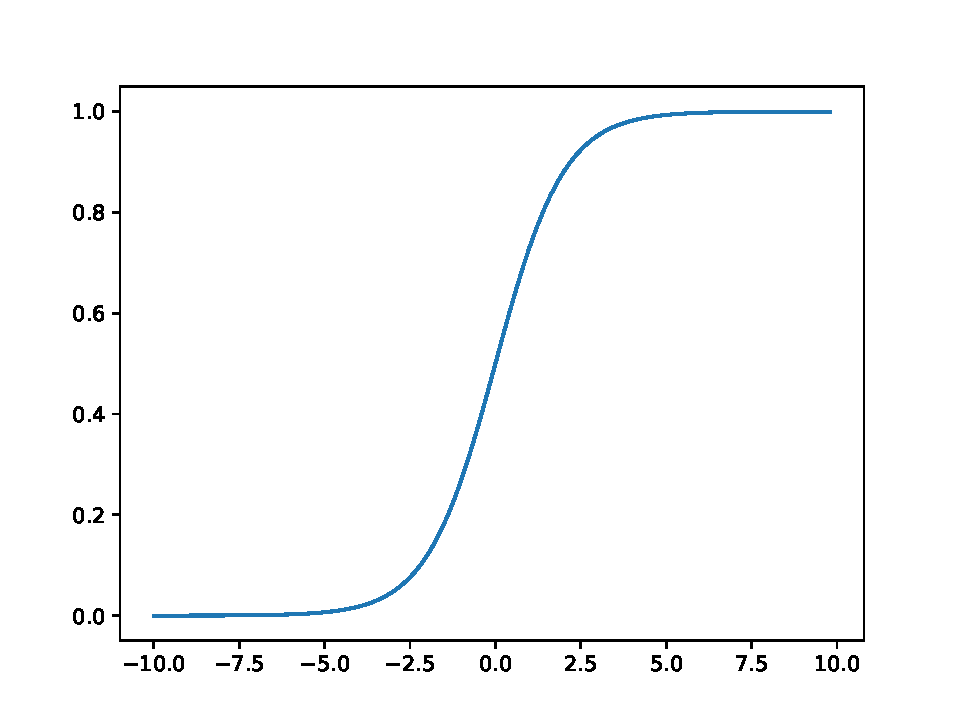
\includegraphics[scale = 0.7]{figures/machineLearning/sigmoid.pdf}
                \caption{Sigmoid function, as can be seen it outputs a value between 0 and 1, $h_\theta(x) \geq 0.5$ is classified as $1$, $h_\theta(x) < 0.5$ is classified as $0$}
                \label{fig:sigmoid}
            \end{figure}
            
            
            
            % \begin{align}
            %     err(h_\theta(X),y) = 
            %     \begin{cases}
            %         1 &\text{if } h_\theta(X),y) \geq 0.5 \text{ and } y = 0 \text{ or } h_\theta(X),y) < 0.5 \text{ and } y = 1 \\
            %         0 &\text{else}
            %     \end{cases}
            % \end{align}
            
    
            
        
            \subsubsection{Support vector machines}
            
            Support vector machine or SVM, can be used for both supervised and unsupervised learning. In the unsupervised case, it is most commonly used for outlier and boundary detection. For supervised learning it handles two classes at a time, so one vs the rest is used if there are more than two classes. The classifier defines a hyperplane that separates the two different classes. The hyperplane can then later be used to predict which class a new feature vector belongs to.  
            
            In general SVM follows the same patterns as the regression classifiers explained above. A cost function is minimized by finding the gradient of it, and the parameters are updated accordingly. Either to convergence or until a given number of iterations are reached. 
            
            SVM is capable of separating data both linearly and nonlinearly. How the algorithm separates the data depends on the kernel function it uses. A kernel function, or a similarity function, describes how similar two feature vectors are by taking the inner product of the two samples in a higher dimensional space. The kernel function does this without having to explicitly transform the data into this dimension. This means that nonlinear shapes can be detected without having to explicitly calculate the new feature space, as is the case with linear and logistic regression. 
            
            A hyperplane is a plane that has one less dimension than the original feature space. So for a two dimensional feature space, the hyperplane becomes a line. By this logic one should not be able to define a complex nonlinear decision boundary for the 2D feature space, but here is where the kernel trick comes to the rescue. 
            
            If the Gaussian kernel
            
            \begin{align}
                K_g(\bm x^{1},\bm x^{2}) = e^{\frac{\norm{\bm x^{1}-\bm x^{2}}^2}{2\sigma^2}} 
                \label{svm:gauss}
            \end{align}
            
            is used, each datapoint in the 2D feature space is transformed into 3D. The third dimension now becomes the evaluation of the kernel function. Hence the hyperplane that now separates the two classes becomes a 2D plane. The choice of $\sigma$ for the Gaussian kernel is important when looking into over- and underfitting. 
            
            The polynomial kernel,
            \begin{align}
                K_p(\bm x^{1},\bm x^{2}) = (\bm x^{1T}\bm x^{2} + \alpha)^\beta,
                \label{svm:poly}
            \end{align}
            
            is another example of a kernel function. Here $\beta$ correspond to the polynomial degree and $\alpha$ is a bias term. These are just two of many examples. The Gaussian or RBF kernell is a good first choice if you know that you have a nonlinear boundary, but don't know exactly what shape the boundary will take. If you have more knowledge about the shape of the boundary you are looking for, you might want to consider more special kernels.
            
            The following mathematical derivation is based on \cite{Hastie}, and a more thorough explanation can be found in its chapters 4.5 and 12. The main goal is to give the reader an intuition on how the algorithm works. 
            
            \begin{align}
                f(\bm x) = \beta_0 + \bm \beta^T\bm x = 0,
                \label{svm:hyper}
            \end{align}
            
            
            defines a hyperplane. For any two feature vectors $\bm x^{[1]},\bm x^{[2]}$ that lie in or on the hyperplane where $\bm \hat x = \bm x^{[1]} - \bm x^{[2]}$, gives  $\bm \beta^T \bm \hat x = 0 $ and hence, $\bm \beta$ is a scalar multiplication of the normal vector to the hyperplane, 
            
            
            \begin{align}
                \bm \beta^* = \frac{\bm \beta}{\norm{\bm \beta}}.
                \label{svm:norm}
            \end{align}
            
             When inserting any feature point $\bm x_0$ that lies on or in the hyperplane defined by Equation \ref{svm:hyper}, one get $\bm \beta_0 + \bm \beta^T\bm x_0 = 0$ which yields $\bm \beta^T\bm x_0 = -\bm \beta_0$. 
            
            
            
            By using $\bm x_0$ as any feature vector from origo to the hyperplane and the normal vector $\bm \beta^*$, the distance for any given feature vector $\bm x$ to the hyperplane is given by
            
            \begin{align}
                \bm \beta^{*T}(\bm x - \bm x_0) = & \frac{\bm \beta^T}{\norm{\bm \beta}} (\bm x - \bm x_0) \nonumber \\
                = & \frac{1}{\norm{\bm \beta}}(\bm \beta^T\bm x- \bm \beta^T\bm x_0) \nonumber \\
                = & \frac{1}{\norm{\bm \beta}}(\bm \beta^T\bm x + \bm \beta_0) \nonumber \\
                = & \frac{1}{\norm{f'(\bm x)}}f(\bm x).
                \label{svm:dist}
            \end{align}
            
            
            
            A decision rule 
            
            \begin{align}
                y^i(\bm x^{iT} \bm \beta + \beta_0) \geq 1 
                \label{svm:decision}
            \end{align}
            
            can then be created using the hyperplane. Since there are two classes they are defined as $y_0 = 1$ and $y_1 = -1$. The decision rule tells which class a feature vector belongs to.
            
            
            
            
            
            Now that an expression for the distance from a hyperplane to any given feature vector in the feature space is defined, one can look at how to find the optimal hyperplane to separate the two classes. The margin or the width between the two closest point from both classes can be defined as $M = \frac{2}{\norm{\bm \beta}}$, and hence maximizing the distance can be formulated as minimizing 
            
            \begin{align}
                J(\bm \beta) = & \frac{1}{2}\norm{\bm \beta}^2 \nonumber \\
                 s.t \quad y^i(\bm \beta^T\bm x^i + \beta_0) \geq & 1 \quad \forall \enspace i.
                \label{svm:cost}
            \end{align}
            
            The constraint here ensures that every point is classified correctly.
            
            \begin{align}
                L = \frac{1}{2}\norm{\bm \beta}^2 - \sum_{i=1}^n \alpha_i[y^i(\bm \beta^T\bm x^i + \beta_0) - 1]
                \label{svm:lagrange}
            \end{align}
            
            shows the equation rewritten as a Lagrangian optimization problem. Setting the partial derivative of $L = 0$, gives the expression

            \begin{align}
                \frac{\partial L}{\partial \bm \beta} = & \bm \beta - \sum_{i=1}^n \alpha_i y^i\bm x^i \nonumber\\
                \bm \beta = & \sum_{i=1}^n \alpha_i y^i\bm x^i, 
                \label{svm:partialbeta}
            \end{align}
            and
            
            \begin{align}
                \frac{\partial L}{\partial \beta_0} =& -\sum_{i=1}^n \alpha_i y^i \nonumber   \\
                \sum_{i=1}^n \alpha_i y^i =& 0
                \label{svm:partialbeta0}
            \end{align}
            
            Inserting Equation \ref{svm:partialbeta} and \ref{svm:partialbeta0} into \ref{svm:lagrange}, gives the Wolfe dual maximization problem,
            
            \begin{align}
                L = \sum_{i=1}^n  \alpha_i - \frac{1}{2} \sum_{i=1}^n \sum_{j=1}^n \alpha_i \alpha_j y^i y^j \bm x^{iT} \bm x^j.
                \label{svm:dual}
            \end{align}
            
            One of the great benefits of the SVM is that the Lagrangian optimization problem defined in Equation \ref{svm:dual} is a convex optimization problem, and hence it has a global maxima.
            
            
            If your classes are not linearly separable in the feature space, maximization of Equation \ref{svm:dual} has no global solution. However as can be seen in Equation \ref{svm:dual} one want to minimize $\bm x_i^T  \bm x_j$. This term can then be replaced by the kernel function defined in paragraph three in this section, which now enables separation in a higher dimensional space.
            
            
            
            
            One interesting observation can be made by inserting Equation \ref{svm:partialbeta} into Equation \ref{svm:decision}. This yields 
            
            \begin{align}
                y^i(\sum_{j=1}^n \alpha_j y^j \bm x^{iT}\bm x^j + \beta_0).
                \label{svm:decision2}    
            \end{align}
            
            Both the decision function and the optimization problem depend only on the pairs of dot product of the x vectors. Which further supports the usage of the kernel functions. The final thing to remark is that not all datasets are completely separable, to deal with this a slack variable is introduced into the optimization to allow miss-classification of some of the feature vectors. 

    
            \subsubsection{Neural networks}
            A neural network attempts to make a machine learn like humans. The algorithm is modeled from how we think the neurons in the human brain learn. A fascinating fact is that a four year old child is better at classifying images than a modern supercomputer. If one could Figure out exactly how the human brain works, and implement a similar learning scheme for computers, only the sky would be the limit. A NN can be look at as an extension of the regression methods described above. In the regression methods the input data $\bm x$ is given to a function $h_\theta(\bm x)$, that either predicts a continuous value, or a class. In a NN, instead of letting $h_{\theta}(\bm x)$ serve as the prediction, the output is used as input for a new layer.
            
            \begin{figure}[h]
                \centering
                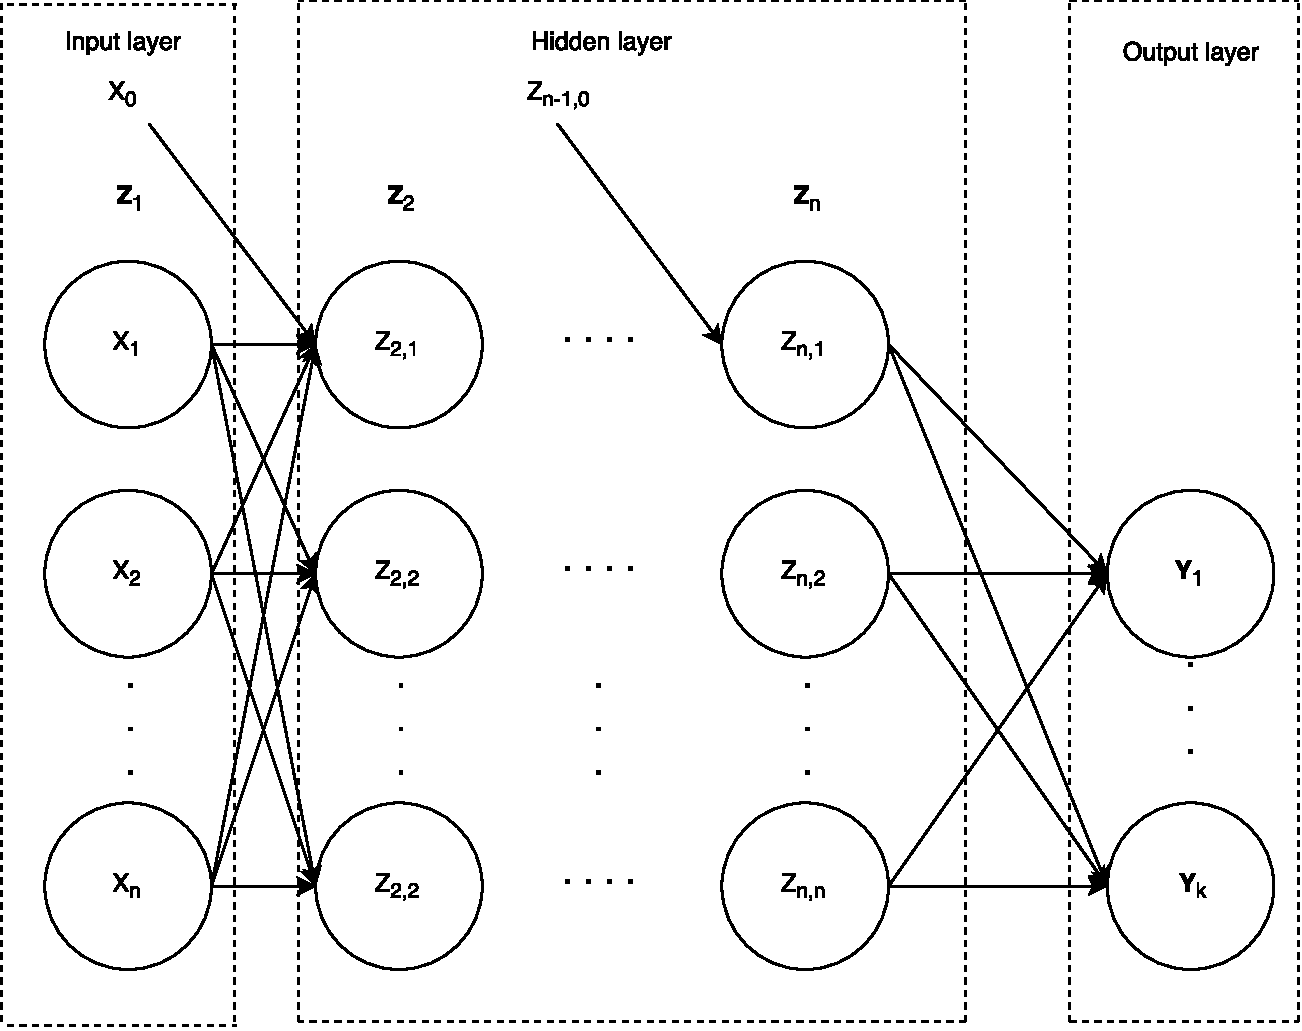
\includegraphics[width=0.8\textwidth]{figures/machineLearning/neural_network.pdf}
                \caption{A graph visualizing a N-level deep neural network}
                \label{fig:nn_fullnetwork}
            \end{figure}
            
            
            
            A NN is a n class classification or regression algorithm. A good visual representation is a graph with nodes and vertices as shown in Figure \ref{fig:nn_fullnetwork}. As seen, a NN consist of three parts. An input layer, a hidden layer and an output layer. The input layer is the feature vectors for the data samples, the hidden layer does all the computation and the output layer does the prediction. A NN with only one layer and a limited number of neurons, can approximate any function \cite{Hastie}. This shows how power full a NN can be. Notice that in Figure \ref{fig:nn_fullnetwork} a bias feature is added to every layer, that is not a part of the original feature set. A NN used for regression, will normally have $k=1$ for the output layer, while a NN for classification will have $k=\textit{\#classes}$. Even if a NN is capable of approximating any function, it does not necessarily mean that it is a trivial task. The more nodes and layers a NN consists of, the harder the network become to interpret. Note that Figure \ref{fig:nn_fullnetwork} have all the outputs from the previous layer, connected to all neurons in the next layer, this is not necessarily the case.
            
            
            \begin{figure}[h]
                \centering
                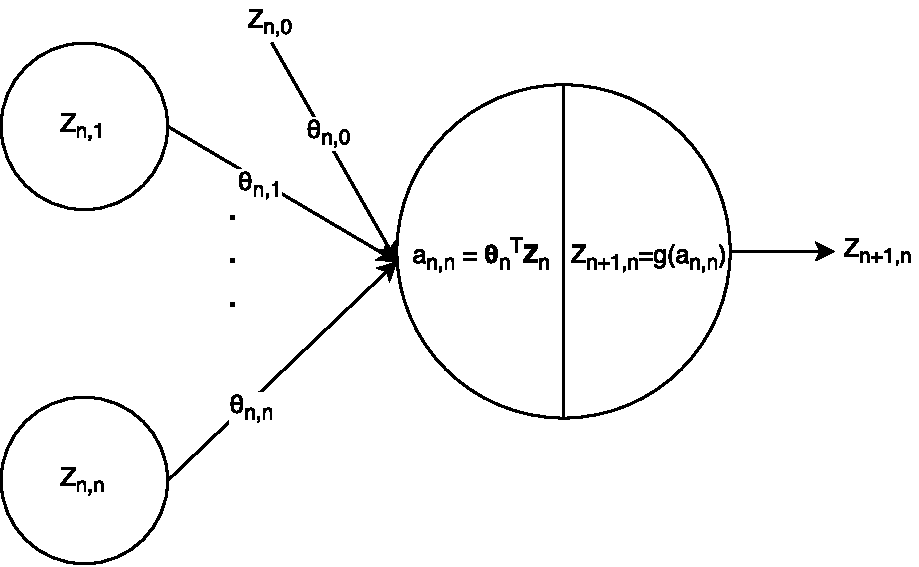
\includegraphics[width=0.5\textwidth]{figures/machineLearning/single_neuron.pdf}
                \caption{Visualization of a single neuron}
                \label{fig:nn_neuron}
            \end{figure}
            
            The following mathematical derivation is based on \cite{Hastie}, \cite{Ng}, and \cite{Nga}. Each of the nodes marked  $z_{n,n}$ seen in Figure \ref{fig:nn_fullnetwork} is what we call a neuron. A single neuron is visualized in Figure \ref{fig:nn_neuron}. Each neuron does two things. First it takes the dot product of the input vector and the weight vector, 
            
            \begin{equation}
                a = \bm \theta_n^T \bm Z_n,
                \label{eq:neuron_a}
            \end{equation}
            
            also shown in Figure \ref{fig:nn_neuron}. Then the output $Z_{n+1,n}$ is calculated 
            
            \begin{equation}
                Z_{n+1,n} = g(a_{n,n}).
                \label{eq:nn_activation}
            \end{equation}
            
            Here $g(a)$ is known as an activation function. There are many different options for activation functions, the most common are shown in Table \ref{tab:acitvations}. If the identity function is used, one can easily verify from Figure \ref{fig:nn_neuron} that a one layer NN is actually the same as regression. When working with classification, the most commonly used activation functions are Relu and Sigmoid/Softmax. All of these functions are nonlinear, and it is by using nonlinear activation functions, that a NN is enabled to approximate any function. If only linear functions are used, it can be verified that adding more layers does not but complicating a linear interpretation \cite{Hastie}. 
            
            
            %%%%%%%%% activation fucntions 
            % \begin{align}
            %     g_k(a) = a \textit{ identity function} \\
            %     g_k(a) = \frac{1}{1+e^{-a}} \textit{ sigmoid function} \\
            %     g_{k}(a) = \frac{e^{Tk}}{\sum_{i=1}^Ke^{Ti}} \textit{ softmax function} \\
            %     g_{k}(a) = \frac{e^a-e^{-a}}{e^a+e^{-a}} \textit{ tanh function} \\
            %     g_{k}(a) = max(a,0) \textit{ relu function}
            %     \label{eg:activations}
            % \end{align}
            
        \begin{table}[h]
            \centering
            \begin{tabular}{ | c | c |}
                \hline
                Function & Function\\ \hline
                Identity & $g_k(a) =a$ \\ \hline
                Sigmoid & $g_k(a) =\frac{1}{1+e^{-a}}$ \\ \hline
                Softmax & $g_k(a) =\frac{e^{Tk}}{\sum_{i=1}^Ke^{Ti}}$ \\ \hline
                Tanh & $g_k(a) =\frac{e^a-e^{-a}}{e^a+e^{-a}}$ \\ \hline
                Relu & $g_k(a) =max(a,0)$ \\ \hline
            \end{tabular}
            \caption{Different activation functions}
            \label{tab:acitvations}
        \end{table}
                    
            % \begin{align}
            %     z_{m} =  \sigma(\theta_{0m} + \bm \theta_m^T \bm z_{m-1}), \textit{m = 1,..,M} \nonumber \\
            %     \bm \hat y = g(\bm z_m) \nonumber \\
            %     \label{eq:fwdprop} 
            %     % \textit{where $\sigma()$ and g() are different activation function}\nonumber 
            % \end{align}
            % In the first layer, $\bm z_1 = \bm x$. For all the other layers each $z_m$ is given by the activations function of a bias term pluss the dot product of the inputs $\bm z$ and the weight $\bm \theta$. This means that for each layer there exists $m$ $\bm \theta$ vectors, which can be written as $\bm \Theta_m$. For the regression classifiers one only had one vector $\bm \theta$, but for a NN you end up with $m$ $\bm \Theta$ matrices. This gives a good indication on why a NN can approximate any given function. 
            
            In the final layer, the output $\hat y$ is calculated. The number of elements in the final layer depends as mentioned if classification or regression is being performed. For regression, the final layer normally only has one element, but for classification, it holds as many elements as there are classes. For binary classification, the Sigmoid function is normally used. For k-class classification, the Softmax function is used, and for regression the identity function. 
            
            
            
            The iteration through the NN mentioned above, is known as forward propagation. It takes a feature vector as input, process it through the layers and either predicts a class or a value. But this does not explain how the NN is trained. As with the regression methods, the weight or coefficients in $\bm \Theta = [\bm \Theta_1 ... \bm \Theta_n]$ needs  to be updated.  This update step is known as backpropagation. The goal is to minimize a cost function as a function of $\bm \Theta$. The cost function used in a NN depends on whether or not it is regression, binary or k-class classification. The three different options are 
            
            \begin{align}
                E(\bm\Theta) = &\sum_{i=1}^M\frac{1}{2}(\hat{y} - y)^2 \nonumber\\
                E(\bm\Theta) = & -\sum_{i=1}^M(y\log(\hat{y})+(1-y)\log(1-\hat{y}) \nonumber\\
                E(\bm\Theta) = &- \sum_{i=1}^m \sum_{k=1}^K y_{ik}\log(\hat y),
                \label{nn:cost}
            \end{align}
            
            
            for a training set of size M. For k-class classification the inner summation is over all the classes. It is not only important to verify that the correct class is predicted, it is equally important that not any of the other classes are wrongly predicted.
            
            
            
            
            The same approach is used for minimizing $E(\bm \Theta)$ as for the previous methods. Gradient descent or another optimization algorithm is used to calculate each of the different parameters in $\bm \Theta$'s contribution to the cost. $\bm \Theta$ is updated as 
            
            \begin{align}
                \bm \Theta := & \bm \Theta - \alpha \nabla E(\bm \Theta) \nonumber \\
                \Theta_{ij} = & \Theta_{ij} - \alpha \sum_{k=1}^M \frac{\partial E_k}{\partial \Theta_{ij}} 
                \label{bp:1}
            \end{align}
            
            Here $\alpha$ is the learning rate, as described in a previous section. As can be verified by the equations in \ref{nn:cost}, the total cost increases when a prediction does not match the given label.
            
            
            The intuitive explanation to what the backpropagation does, is that the prediction errors, can be back-propagated to calculate the error in each neurons prediction. This prediction error is then used to update the corresponding weights for the neuron in matrix $\bm \Theta$. The partial derivative of the cost function is defined as
            
            % Equation \ref{bp:1} to \ref{bp:9} shows how the partial derivative of the cost function is computed.   
            
            \begin{align}
                \frac{\partial E}{\partial \Theta_{ji}} = \frac{\partial E}{\partial a_{ji}} \frac{\partial a_{ji}}{\partial \Theta_{ji}} \label{bp:2}.
            \end{align}
            
            Solving for the first term,
            \begin{align}
                \delta_{ji} \coloneqq \frac{\partial E}{\partial a_{j,i}} = \sum_{k=1}^N \frac{\partial E}{\partial a_{j+1,k}} \frac{\partial a_{j+1,k}}{\partial a_{ji}} \label{bp:3}
            \end{align}
            
            where
            
            \begin{align}
                 \frac{\partial E}{\partial a_{j+1,k}} = \delta_{j+1,k}
            \end{align}
            
            and
            \begin{align}
                \frac{\partial a_{j+1,k}}{\partial a_{ji}} = \frac{\partial \bm \theta_{j+1}^T \bm Z_{j+1}}{\partial a_{ji}}. \label{bp:4}
            \end{align}
            
            $\bm \theta_{j+1}^T \bm Z_{j+1}$ can be written as, 
            
            \begin{align*}
                \bm \theta_{j+1}^T \bm Z_{j+1} = \Theta_{j+1,0}Z_{j+1,0} +\textit{ }..+ \textit{ }\Theta_{j+1,N}Z_{j+1,N} \nonumber \\
                = \Theta_{j+1,0}g(a_{j,0}) + \textit{ }.. +\textit{ }\Theta_{j+1,N}g(a_{j,N}). \label{bp:5}
            \end{align*}
            
            This gives, 
            \begin{align}
                \frac{\partial a_{j+1,k}}{\partial a_{ji}} = \Theta_{j+1,i}\frac{\partial g(a_{j,i})}{\partial a_{ji}} =  \Theta_{j+1,i}g'(a_{ji}), \label{bp:6} 
            \end{align}
            
            which finally yields
            \begin{align}
                \delta_{ji} = g'(a_{ji})\sum_{k=1}^N\delta_{j+1,k}\Theta_{j,k}. \label{bp:7}
            \end{align}                    
            
            Solving for the second term
            \begin{align}
                a_{ji} = \bm \theta^T_i \bm Z_{i} \label{bp:10}
            \end{align}
            
            \begin{align}
                \frac{\partial a_{ji}}{\partial \Theta_{ij}} =  Z_{ji} \label{bp:8}
            \end{align}
            
            Gives the following equation
            \begin{align}
                \frac{\partial E}{\partial \Theta_{ji}} = \delta_{ji}Z_{ji} \label{bp:9}
            \end{align}
            
            
            
            
            The forward and backwardpropagation steps are then iterated over until a given number of iterations are reached. A complete pass forward and backward of all training examples, is known as one epoch. When the training set is large, it is often split into smaller batches to speed up calculations. The batch size tells you how many samples should be included in each forward and backward pass. Splitting the data into batches enables the algorithm to take advantage of parallelism, running the separate batches on separate CPU's or GPU's. Notice in Equation \ref{bp:9} that $Z_{ji}$ is a part of the expression. This term is calculated as a part of the forward propagation, hence when developing a NN storing these values will reduce the computation time. 
    
                
            When you design a NN, you are free to make it as wide and deep as you want. However, the deeper you make it, the more processing each iteration through it will take. Deep networks also increases the risk of overfitting. A good approach is to start with a shallow network, and increase the depth and width until you see that adding new layers, does not yield better performance. To avoid overfitting the regularization term 
            
            \begin{align}
                \frac{\lambda}{2} \sum_{km} \Theta_{km}^2  \nonumber \\
                = \frac{\lambda}{2}\bm \Theta^T \bm \Theta,
                \label{nn:overfit}
            \end{align} 
            
            is added to the cost function. The extra term in the cost function will penalize parameters $\neq 0$.   
            
            
            This slightly modifies the update rule as 
            
            \begin{align}
                \bm \Theta = & \bm \Theta - \alpha \nabla E(\bm \Theta) - \alpha \frac{\lambda}{2} \frac{\partial \bm \Theta^T \bm \Theta}{\partial \bm \Theta} \nonumber \\
                = &(1-\alpha \lambda)\bm \Theta - \alpha \frac{\partial E(\bm \Theta)}{\partial \bm \Theta}.
                \label{nn:updaterule2}
            \end{align}
            
            Since the regularization term is introduced to reduce the weights in the NN, it is a natural conclusion that the weights should be initialized to small values. Zero initialization is however not a good option, this will lead to zero derivatives, and hence the model will never be updated. Initializing all weights to a random number near zero, will give a roughly linear model \cite{Hastie}. This means that the model will start out more or less as a linear function and will grown in nonlinearity if necessary. 

    \subsection{Scikit-learn}
    Scikit-learn \cite{scikit-learn}, \cite{scikit-web} is an open source toolbox available for Python. It includes a number of different machine learning algorithms and the tools needed to preprocess and analyze your data. The framework created by scikit-learn is used throughout this project, mainly because it either includes the algorithms that are to be tested, or there exist an API that allows you to run the non existing algorithms through the scikit-learn framework. 
    
    In addition to the being a great machine learning library for Python, the website \footnote{\url{http://scikit-learn.org/stable/ }}also explains the main theory behind the different algorithms, and what the scikit-learn algorithms are built upon in a easy to find manner. This makes it a good choice when one want to understand what is making the algorithms work.        
    
    \subsection{Keras}
        Scikit-learn does not include neural networks. Different libraries were considered before Keras was chosen for the NN analysis. Keras \cite{chollet2015keras} is a Python library that simplifies creation of NNs in Python. Instead of having its own implementation of NNs, it uses other NN python libraries as backends. This means that you can run you analyzis using for example Google's TensorFlow through Keras. At this moment Keras supports Google's TensorFlow, Theano developed by LISA Lab at Université de Montréal and CNTK developed by Microsoft. This means that by using Keras, only one line of code needs to be changed if one want to change between one of the options above. Developing code using one of the NN libraries directly would make switching between the different options more cumbersome. However, one important factor to keep in mind, is that Keras is not officially supported by any of the backend developers. This means that  not all of the original functionality is guaranteed to be supported in Keras. Regardless, the fact that Keras is easy to use and its focus on enabling fast experimentation, are the main reasons for developing in Keras. Keras supports the normal sequential NN which is used in this analysis, but it also has support for the more complex convolutional and reccurent NN. It can also run on both CPU and GPU, making it flexible and optimizable to the hardware it runs on. More information about Keras can be found at \footnote{\url{https://keras.io/}}.
            
        \subsubsection{Google TensorFlow}
            For this project only the TensorFlow backend is tested. TensorFlow \cite{Abadi} is developed by The Google Brain project, and it started as the DistBelif project back in 2011. Tensor flow is the second generation, built upon the experiences from DistBelif. Tensorflow has support for parallelism and has the possibility to have many different devices collaborating on the same problem. As stated in \cite{Abadi}, "a computation expressed using TensorFlow can be executed with little or no change on a wide variety of heterogeneous systems, ranging from mobile devices such as phones and tablets up to large-scale distributed systems of hundreds of machines and thousands of computational devices such as GPU cards". This shows the flexibilty TensorFlow introduces. More information about TensorFlow can be found at \footnote{\url{https://www.tensorflow.org/}}.
        
        
        
    % \subsection{Evalutation of the classifiers}
    
    %     \subsubsection{F1 score}
    %     \subsubsection{accuracy}
    %     \subsubsection{Learning curves}
    %     \subsection{Visual checking}
        
        
        
    \subsection{How the different algorithms are analyzed}
        \subsubsection{Prediction accuracy}
            One way to evaluate the classifiers performance is using the prediction error. An error function for a two class classifier is defined as
            
            \begin{align}
                \err(h_\theta(X),y) = 
                \begin{cases}
                    1 &\text{if } h_\theta(X),y) \geq 0.5 \text{ and } y = 0 \text{ or } h_\theta(X),y) < 0.5 \text{ and } y = 1. \\
                    0 &\text{else}.
                \end{cases}
                \label{eq:error_func}
            \end{align}
            As can be seen, a prediction is classified as wrong if rounding it to the nearest integer $(0,1)$ gives a different value than the data label given by the label set. The test error is then calculated by summing over all pairs $\bm{x_{train}^i}, y_{train}^i$ and calculating the average value by dividing by the number of samples, 
            \begin{align}
                \frac{1}{m} \sum_{i=1}^{m_{test}}\err(h_\theta(x_{test}^i,y_{test}^i).     
                \label{lr:testError}
            \end{align}
            This is used to classify the different logistic regression classifiers, and to pick the best one. One need to take caution when applying a test like this on skewed datasets. If the data set is very skewed, with only a small number of for example negative training examples, then a classifier that predicts $1$ for all data-points will score well on the test error, even if it predicts every negative training example wrong. 
            
            
        \subsubsection{F1 score}
            Prediction error or prediction accuracy are a quick ways to look at your classifiers performance. However, high accuracy does not necessarily mean that your classifier is doing a great job. To deal with the skew issue F1 score is introduced. The F1 score is calculated as
            
            \begin{align}
                F1 = 2\frac{\text{precision}*\text{recall}}{precision+recall}.
                \label{eq:f1_score}
            \end{align}
            
            For this to make sense, the terms precision, 
            
            \begin{align}
                \text{Precision} = \frac{\text{\#TruePositive}}{\text{\#TruePositive}+\text{\#FalsePositive}},
                \label{eq:precision}
            \end{align}
            and recall,
            \begin{align}
                \text{Recall} = \frac{\text{\#TruePositive}}{\text{\#TruePositive}+\text{\#FalseNegative}},
                \label{eq:recall}
            \end{align}
            
            needs to be explained. Equation \ref{eq:precision} and \ref{eq:recall} show how the two different terms are computed, and Table \ref{tab:prerec} explains the different terms
            
            \begin{table}[h]
                \centering
                \begin{tabular}{| p{4cm} | p{4cm} |}
                    \hline
                    Term & Explanation\\ \hline
                    \#TruePositive & The number of predictions classified to the class correctly.\\ \hline
                    \#FalsePositive & The number of predictions classified to the class wrongly. \\ \hline
                    \#FalseNegative & The number of predictions that should have been classified to the class, but are not. \\ \hline
                \end{tabular}
                \caption{Explanation of the terms used to calculate the $F1$ score}
                \label{tab:prerec}
            \end{table}
            
            Hence one should calculate the $F1$ score for all classes, to check a classifiers performance. 
        
        % \subsubsection{Precision recall curve}
        %     To get av more visual representation of the performance on skewed datasets, precision/recall curves can be used. 
        %     Once plotted the graph shows how well the prediction has gone by the area under the curve. The larger the area, the better the performance. create plots for the different lr classifiers, to confirm that performance is increasing until degree 8.
        %     Use the curve to show if it is precision or recall that is large for the F1 score. Since the F1 score is already beeing used to numerically evaluate the performance. 
        
        \subsubsection{Learning curves, bias vs variance}
            The $F1$ score tells you how well your classifier is doing. However, it does not tell you what you should do if it is not yielding sufficient results. This is where learning curves, bias and variance comes into play. A learning curve plots the classifiers performance  on the training and cross validation set, as a function of the training set size. In it simplest form, you split your data into two parts traning and test sets. At first you only use a small subset of the training set to train your classifier. After training you check your classifiers performance on the subset used for training, and also on the test set. The size of the traning set is then increased for each iteration to see if more data yields a better performance. Figure \ref{fig:learning_curves} shows what a learning curve plot can look like. As can be seen the accuracy on both training and test set increase as the number of training samples increases. One important thing to notice is that both training and test predictions follow each other very closely. This is indicates that the test set is not holding much new information compared to the training set, hence the better the algorithm fits the training set, the better it fits the test set.  
            
            \begin{figure}[h]
                \centering
                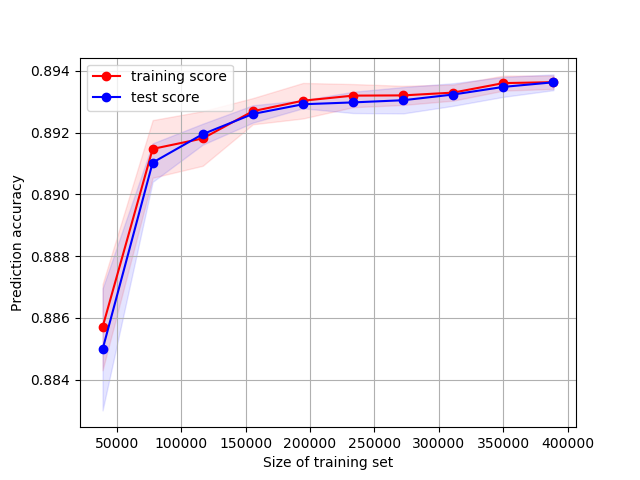
\includegraphics[scale = 0.8]{figures/machineLearning/LearningCurves.png}
                \caption{Learning curve showing the accuracy of the prediction on both test and training sets, as a function of growing training set size}
                \label{fig:learning_curves}
            \end{figure}
            
            Bias and variance are two terms used to describe whether or not the trained classifier is underfitting or overfitting the data model. Underfitting occurs when you try to adapt a too simple model to your data. A good example is trying to fit a line to a circle. No matter how large your training set is, you will never be able to get a good fit between the model and the data. This is known as high bias, and the solution is to use a more complex model. High bias will often give poor predictions on both training and test sets. Variance is on the opposite side, high variance means that you are overfitting the data. No real life dataset is perfect, and by using a too complex model or by not having enough training data this can become an issue. High variance can often be confirmed with a much better training prediction accuracy than test prediction accuracy.  

        \subsubsection{Finding the best parameters for your classifier}
            When you are using one of the ML algorithms to create a classifier, there is a number of parameters you can set, to adjust how the algorithm perform. This is known as hyperparameterization. The basic way to do it, is to create a number of classifiers for the different combinations of input parameters, and to split your dataset into a training and cross validation set. You then use the prediction accuracy on the cross validation set, to determine which of the parameter combinations that yields the best result. To implement this yourself, is however a cumbersome thing, and it would take a lot of time. In this project, a built in method from the scikit-learn library is used instead. 
            
            There are two main approaches, Grid Seach and Randomized search. In most cases Grid Search is performed as an exhaustive search, meaning that it checks all possible combinations of the hyperparameters, to find the best fit. Randomized search, randomly picks a a subset of the parameters for n given iterations, and the best ones are kept. This will drasticly reduce computation time when the number of parameters are large. According to \cite{BergstraJAMESBERGSTRA2012} randomized search performs as well as grid search when the number of parameters grows large, and does so in a much faster manner. Therefor the latter is used.
            
        
        
    % \subsection{PyTorch?}
    %     PyTorch is an alternative to Tensorflow when you want to use neural networks for deep learning. It is a relatively new framework, but is beeing developed fast. Many experts also claim that Pythorch will exist alongside Tensorflow for a long time. Pytorh

    
    
    % \subsection{Preprocessing of data}
    %     The dataset used in this project, has a lot of common data areas. As mentioned, the goal is to enable prediction of a servo indicator's state, based on process signals. The datasets are extremely large, but many of the datapoints does not include any new information, they are simply overlapping other data points, or are from a data set which all servo indicators can generate independent of their current state. Hence one can argue that it would be beneficial to remove those data points to simplify the data analysis. 
        
    %     Need to show plots of the data sets, and explain why this actually is a fact. 
        
    %     \subsubsection{Feature Scaling}
        
    %     \subsubsection{Mean normalization}
        
            
        
    %     \subsubsection{Load reduction}
    %         This section is intended to explain why some of the data points in the data sets are complicating the analysis without adding more information. The power output of the hydro electric power station is controlled by the power consumption of the grid. Increase or decrease in power production is controlled by controlling the flow of water into the turbine, this is again controlled by the servo indicators. When the $\Delta P$ is large enough, this means that $\Delta Flow$ need to change accordingly. When the servo indicators change from steady state to closing or opening, you get hysteresis, which can be seen in the figure. The issue with the data points that are sampled during this hysterisis is that they are common for all servoindicators, both new and old. Hence you are not able to directly observe wether or not the data point should belong to one class or the other. Of course there might be information hidden in the data that you cannot observe in the figures, that can be picked up by a deep neural network. Therfore the emphasis in this project is to check performance between heavily preprossed data, and simple classifiers vs scaled raw data using deep neural networks. 
            
    %     \subsubsection{Median filter}
    %         The first filter used to remove datapoints which fall into the above category is median filter. As can be seen in the figure, it also removes datapoints not related to a change of direction, but it significantly removes the data points in focus, and also reducec the number of data points in the data set. 
            
    %         The median filter is a rolling filter. As the name implies it uses the median of a data set. The clue here is that it takes the median of a given window of the total data set at a time. This enables you to find the median for a subset of the data, calculate the median, and remove outliers, hence datapoints that have a large rate of change. 
            
    % \subsection{Hyperparameter optimization}
        
        
        
    % \subsection{Classifier evalutation}
    
    %     As can be seen, a prediction is classified as wrong if rounding it to the nearest integer $(0,1)$ gives a different value than the data label given by the label set. The test error is then calculated by summing over all pairs $x_{train}^i, y_{train}^i$ and calculating the average value by dividing by the number of samples as can be seen in \ref{lr:testError}. 
    %         \begin{align}
    %             \frac{1}{m} \sum_{i=1}^{m_{test}}err(h_\theta(x_{test}^i,y_{test}^i)     
    %             \label{lr:testError}
    %         \end{align}
    %     This is used to classify the different logistic regression classifiers, and to pick the best one. One need to take caution when applying a test like this on skewed datasets. For the datasets used here, there are the same number of negative and positive training examples. This is done by only picking the same amount from both sets of data. If you however have a very skewed data set, with only a small number of for example negative training examples, then a classifier that predicts $1$ for all datapoint will score well on the test error, even if it predicts every negative training example wrong. 
        

\section{The turbine datasets and preprocessing steps }
    The data used is taken from a large Norwegian hydro electric power plant, shown in Figure \ref{fig:kvilldal} and is provided by Hymatek Controls. This plant has four identical Francis turbines, but with different maintenance history. Instead of using it as four different turbines, it is assumed that the data can be looked at as data from one turbine over a longer time period. This is of course not an ideal case, but shows one of the issues one can encounter when using data based methods. You seldom have all the data you need, and you must either add artificial data, or assume that data from other cases can be used. This is used as an assumption on how process signals from a single Francis turbine will evolve over time, as the turbine is worn down. The data collect for this project was collect during a commissioning period of the plant, meaning that it is only sampled over shorter time periods. In addition, at commissioning, a lot of tests are performed to ensure that the equipment is working as it should. One concrete example is that it can handle fast load reductions. This means that the data available most likely holds much larger variations than what would be seen for data sampled over a longer, but normal operation period.   
    
    \begin{figure}
        \centering
        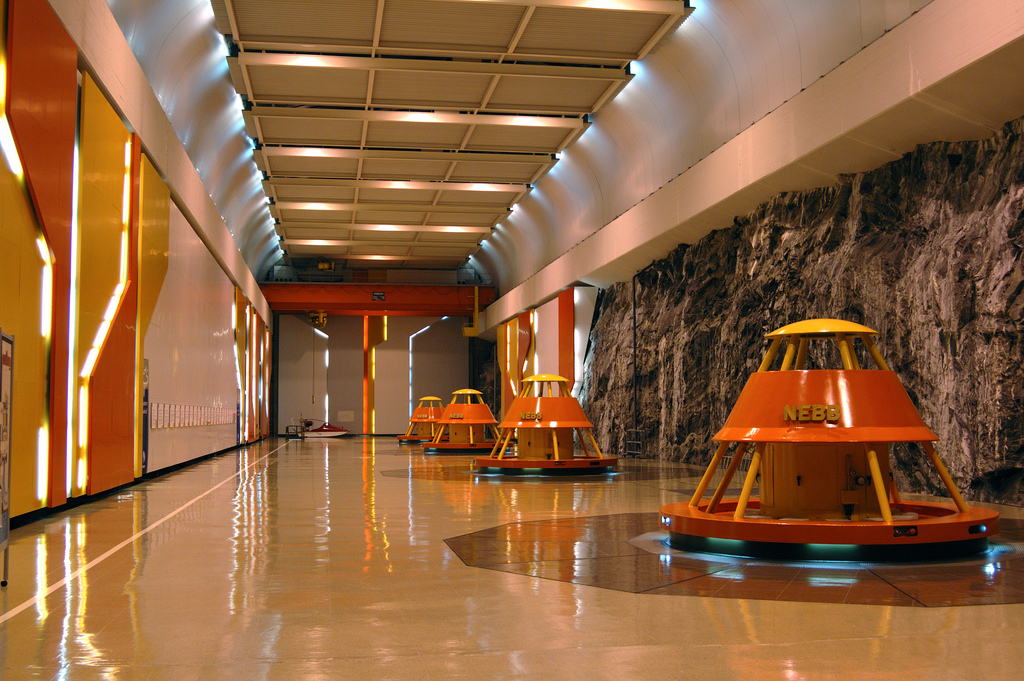
\includegraphics{figures/introduction/Kvilldal.jpg}
        \caption{Top view of the four generators at the actual plant. Courtesy of Statkraft}
        \label{fig:kvilldal}
    \end{figure}
    
    
    Table \ref{tab:variables} explains the features in the original data set.
    \begin{table}[h]
        \centering
        \begin{tabular}{|c|c|}
             \hline
             \textbf{feature} & \textbf{Interpretation}  \\ \hline
             CB pos & State of circuit breaker, open/closed  \\ \hline 
             Close & percentage(0-100\%) of closing pressure on the closing servo motor \\ \hline 
             F [Hz] & Desired output frequency in Hz \\ \hline
             F.err [Hz] & Error in output frequency in Hz \\ \hline
             Open & percentage (0-100\%) of closing pressure on the closing servo motor \\ \hline
             Sjakt & Shaft pressure (0-100\%)\\ \hline
             $Y$ [percent] & Opening of guide vanes in percent (0-100\%)\\ \hline
             $Y_{sp}$ [percent] &  Set point of opening of guide vanes in percent (0-100\%)\\ \hline
             
        \end{tabular}
        
        \caption{Table explaining the different features provided from the plant}
        \label{tab:variables}
    \end{table}
    
    
    \subsection{Original data}
        Figure \ref{fig:timeseries_A2} shows a timeseries plot  for one of the Francis generators. As can be seen the range of the Y axis is large. This is because some of the signals in the feature set have values between $0$ and $100$. This illustrates one important factor when working with data. The feature with the largest value range, will define the scale of the plot, meaning that there can be dynamics not possible to observe in this plot. This issue needs to be taken into consideration when the data is going to be used to build models. Pre-processing is a vital part of data analysis, a feature with a small range, can hold as much or more information as features with higher range. As can be seen, it is hard to interpret much from this plot. This is another very important factor to keep in mind when working with data based methods. Knowing how to make the most of the available data can make a big difference.  
        
        \begin{figure}
            \centering
            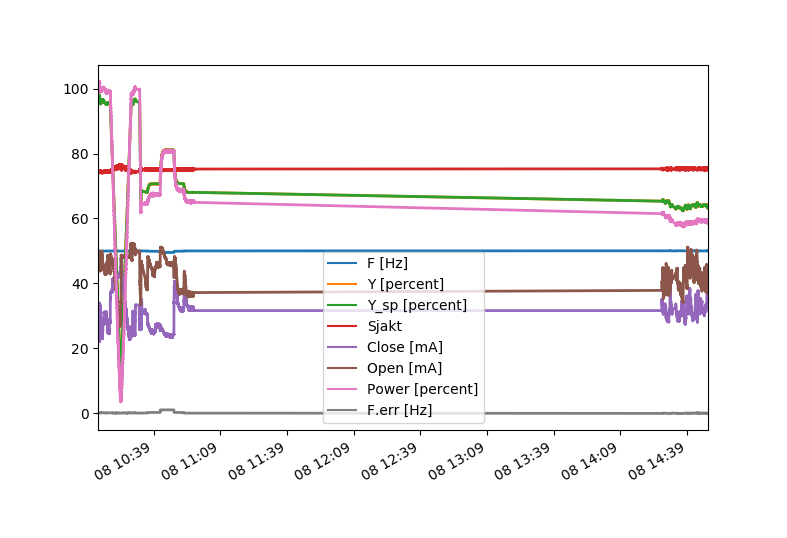
\includegraphics[width=\textwidth]{figures/data/A1_all_timeseries.png}
            \caption{Time series plot for one of the Francis turbines. Here all the original features are plotted as a function of time.}
            \label{fig:timeseries_A2}
        \end{figure}
    
    \subsection{Feature engineering}
        
        "Feature Engineering Is The Key" and "So there is ultimately no replacement for the smarts you put into feature engineering" from \cite{Domingos2012} are two very relevant quotes for this section. Good feature engineering can be the difference between success and failure when it comes to machine learning. Feeding your raw data straight into a learning algorithm is seldom the best choice. The article also discusses the difficulty with intuition in high dimensions and how generalization becomes harder as the feature set grows.     
        
        \begin{figure}
            \centering
            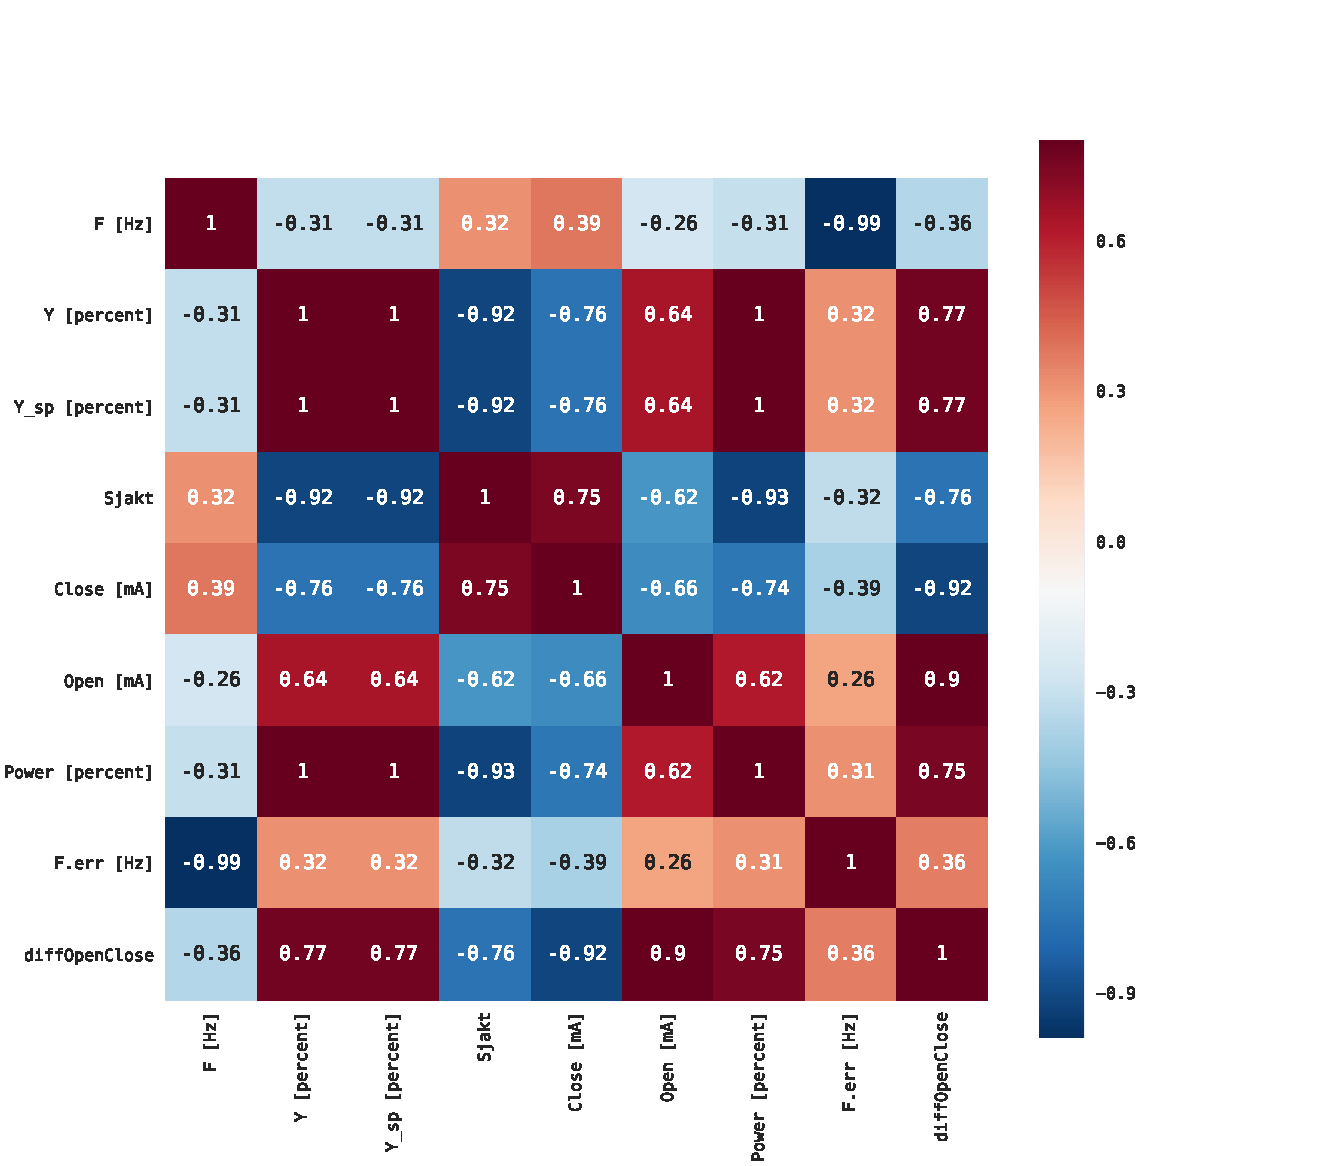
\includegraphics[width = \textwidth]{figures/data/heatmap.pdf}
            \caption{Heatmap showing the correlation between the different features in the data set.}
            \label{fig:heatmap}
        \end{figure}
    
        The heatmap in Figure \ref{fig:heatmap} shows the correlation between the different features in the data set. This is used to analyze which features that introduce new variance to the data set, and which can be explained by already existing features. The heatmap  is used to reduce the number of features that should be used in the analysis. This is known as feature extraction. The complexity of an analysis grows with the number of features, meaning that a reduced feature space, can help speed up the modeling. In the figure, where each column meets each row, a square is formed. The color and value of that square explains how the two features are correlated. A red color with a number close to one indicates that the two features are positive correlated. A dark blue color with a value close to minus one indicates negative correlation. Whine and close to zero indicate no correlation.  
        
        As mentioned in the introduction, the goal is to classify the condition of the guide vanes. \textbf{This is found as function of the differential pressure of the open and closing servos}. Hence $Y$, open and close should be the most interesting features in this data set. As can be seen, $Y$ and $Y_{sp}$ are strongly correlated. This is as expected, since the control system is constantly working to keep $Y$ as close to $Y_{sp}$ as possible. Hence, dropping one of these features in the further analysis will not reduce the amount of information found in the data set. A new feature is added, the difference between $open$ and $close$. This is done to see if the two features can be reduced to one. As can be seen in the column for the new feature $diffOpenClose$ in the heat map, it is strongly correlated with open, and strongly negatively correlated with closing. It is therefore chosen as a substitute for the two original features. The two frequency features are observed to have small correlations with both opening and the new $diffOpenClose$ feature. They are however left out of the feature set. The frequency of the power generated by the turbine is controlled by a set point, and hence it makes sense that it holds little information about the degradation of the guide vanes inside the turbine. $Sjakt$ is the last feature to analyze. As can be seen in the figure, it is negatively correlated with both $Y$ and $diffOpenClose$. It might hold some interesting information for the analysis, but the benefit of keeping the feature space in two dimensions, is weighted higher, and hence it is also left out. From now on the data set is only containing $Y$ and $diffOpenClose$ as features.    
        
    \subsection{Splitting the data}
        As mentioned in the introduction, the state of the guide vanes is by the current approach estimated by analyzing a servo indication of the turbine. Therefore the servo indication is separated from the rest of the commissioning data. This enables analysis on the pure servo indication. The two different datasets will be referenced as \textbf{commissioning} and \textbf{servo indication} from now on. This also introduce the possibility to compare if it is possible to extract the servo indication information from a commissioning or not. Figure \ref{fig:start_up_4} shows the commissioning data for the four different data sets. The $Y$ axis named delta force, is the diffOpenClose feature added to the data set. As can be seen, A3 is the set with lowest differential and A4 is the one with the highest. Figure \ref{fig:start_up_1}, shows the four different data sets plotted against each other. One clear issue is that the A1 set does not span as far as the three others. This is again an example of issues when working with real data. Sometimes one does not have available what one should have. From Figure \ref{fig:start_up_4} and \ref{fig:start_up_1} one can clearly now see the influence of feature engineering compared to Figure \ref{fig:timeseries_A2}. Figure \ref{fig:servo_indication_all} shows the data from the servo indications for the four different turbines. Here one can more easily interpret the four sets in one plot, so a plot for each one individually is left out. One important thing to notice is that the servo indications holds only the information one actually want when estimating the state of the guide vanes, there are only samples that lay on the boundary. Compared to the commissioning sets seen in Figure \ref{fig:start_up_4} where there are a lot of samples located inside the boundary. 
        
        \begin{figure}[h]
            \centering
            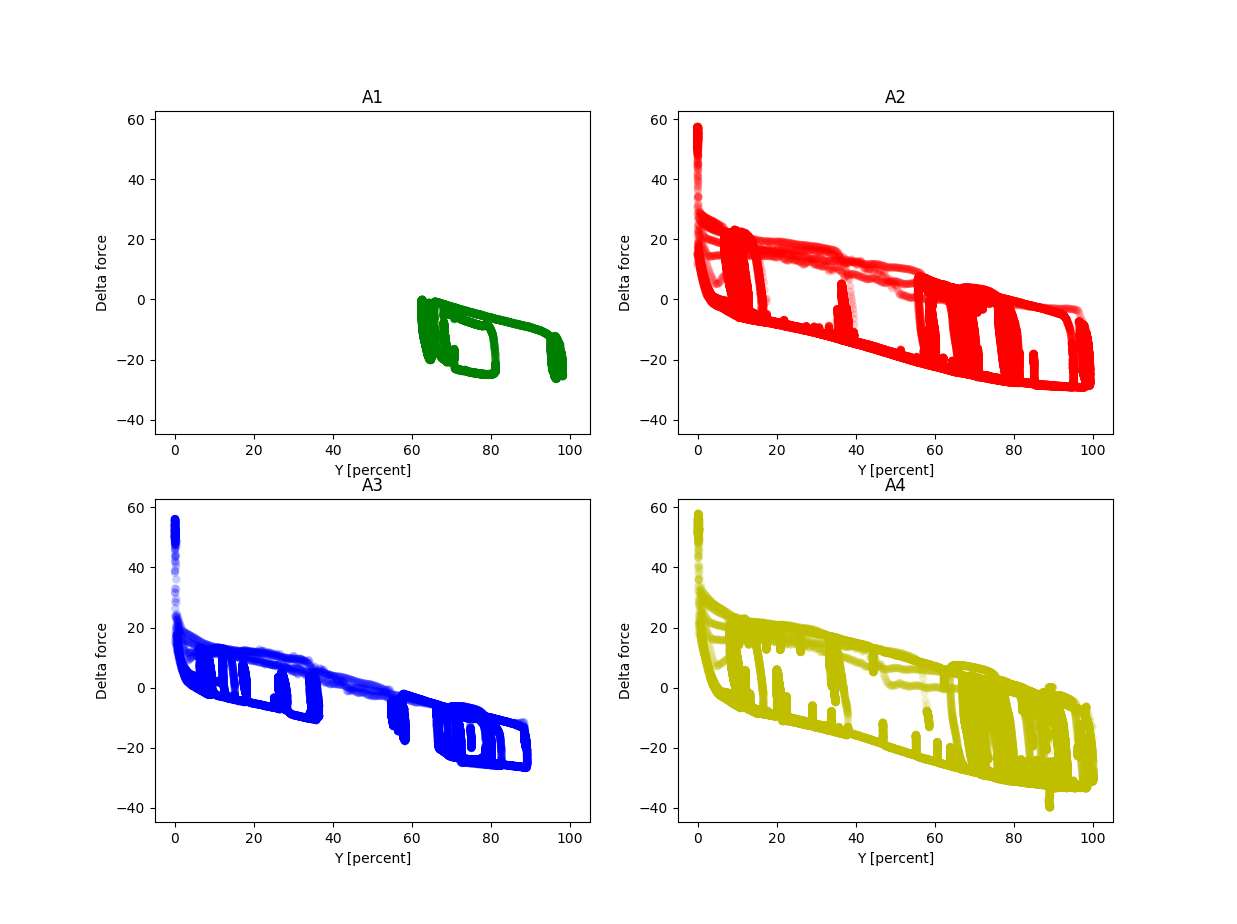
\includegraphics[width = \textwidth]{figures/data/start_up_all.png}
            \caption{Commissioning data for the four turbines. High non linearity can be observed in the left part of the subplots for A2-A4. Also notice that the test data for A1 is very reduced compared to the others. The numerical values of the delta force axis does not correspond to any SI units, it just serves as a factor that can be used to separate the different sets}
            \label{fig:start_up_4}
        \end{figure}
        
        \begin{figure}[h]
            \centering
            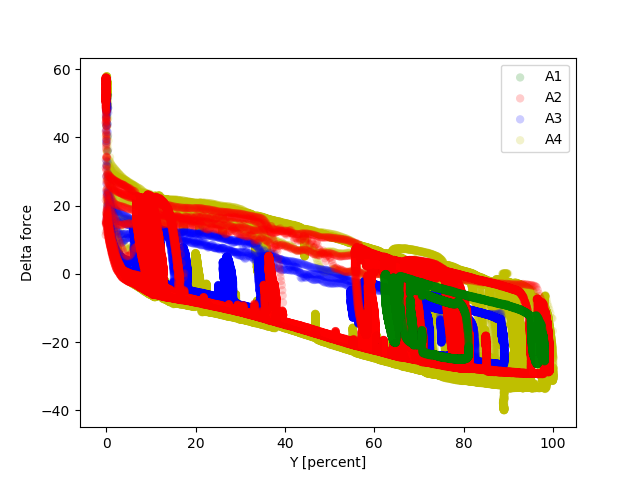
\includegraphics[width = 0.6\textwidth]{figures/data/start_up_all_one_plot.png}
            \caption{The four test sets plotted in the same window. Due to the large amount of samples, and the overlapping samples some of the turbine samples are hidden. It is however possible to verify that A4 is the set with highest delta force, and A3 ist the one with lowest.}
            \label{fig:start_up_1}
        \end{figure}
    
        \begin{figure}[h]
            \centering
            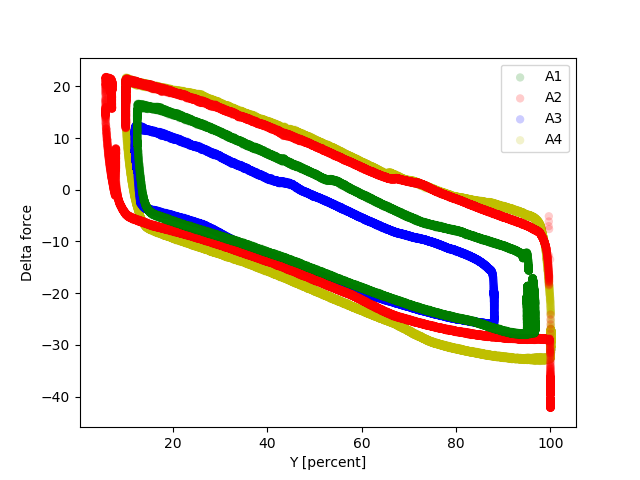
\includegraphics[width = 0.6\textwidth]{figures/data/servo_indication_all_one_plot.png}
            \caption{The four servo indications plotted in the same window. The pure servo indication does not contain any samples inside the boundary area, making the scale of the different turbine data sets easier to interpret. A3-A1-A2-A4 from good to poor.}
            \label{fig:servo_indication_all}
        \end{figure}
        
        
    \subsection{Preprocessing}
        Once the feature space is reduced and the data sets are split, the next step is to preprocess the data, making sure that it is suitable for a learning algorithm. The data for the $4$ different cases comes in several .csv files, sampled during commissioning. I want to thank my supervisor Anders from Hymatek for providing a Python API that reads the files from .csv into python. Figure \ref{fig:start_up_4} shows as mentioned in its caption high nonlinearity in the left part of the plot. This makes the boundary more complex, and it holds little information about the guide vanes. Therefore the samples that lay in this space are removed from the dataset.    
        
        
        \subsubsection{Downsampling}
            The sample rate for the data is 50 Hz, meaning that every $20$ms a new sample is taken. Even for a shorter time period, this yields an enormous amount of samples. Figure \ref{fig:downsample} shows Kde plots for the original and down sampled data set for turbine A4. Kde or kernel density estimation is a way to estimate the probability density function of variable or feature. The Kde for both features are shown above and to the right of the plots. The red color around the samples indicates where the highest density of samples are. This means the plots clearly show where most of the data is located. 
            
            The left figure shows the plot for the commissioning dataset for turbine $4$. The original commissioning set has a sample size of $133700$ samples. The right plot has the sample rate reduced to $1$s, reducing the sample set size to $10756$. Note that there are some holes in the sampling, meaning that there are seconds which not have 50 samples. This is the reason for the unbalance between the number of samples in the original vs the down sampled dataset. As can be seen in Figure \ref{fig:downsample} the shape of the  correlation curves are very similar for both plots. One can also verify that the contours of the original set is still a part of the down sampled plot. This means that even if the amount of data is reduced, it still includes the same shape and density as the original data. Therefor the reduced data sets are the ones used for the analysis. The corresponding plots for the three remaining data sets are found in \textbf{appendix A}. The p value in the upper right corners, indicates the probability of an uncorrelated dataset producing a dataset that has a pearsonr correlation as high or higher as the set. The pearsonr measures the pearsonr correlation, which is a a measure of the linear correlation between the two features    
        
            \begin{figure}[h]
                \begin{minipage}[b]{0.5\linewidth}
                    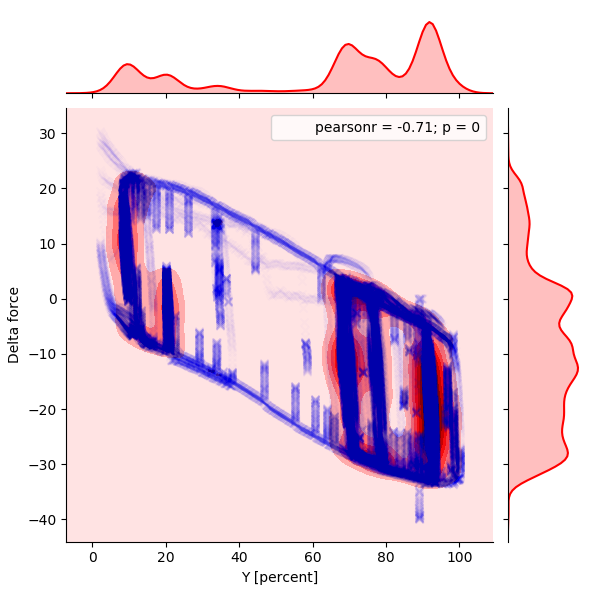
\includegraphics[width=1\linewidth]{figures/data/kdePlot_noServo_A4.png} 
                \end{minipage}
                  \hfill
                  \begin{minipage}[b]{0.5\linewidth}
                    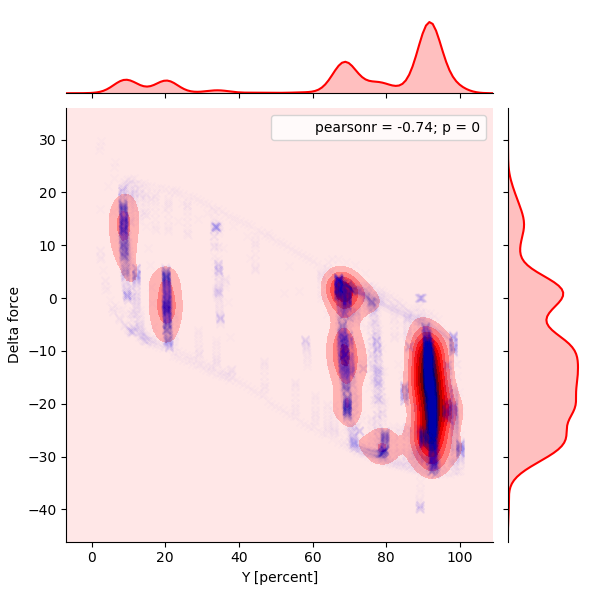
\includegraphics[width=1\linewidth]{figures/data/kdePlot_reduced_noServo_A4.png} 
                \end{minipage} 
                \caption{Kde plots for original commissioning data, and down sampled commissioning data for turbine $4$.}
                \label{fig:downsample}
            \end{figure}
        
            For the servo indication sets, the Kde plot for A4 is seen in Figure \ref{fig:kde_servo}. As can be seen here the data is uniformly distributed around the boundary. The size of the servo indication sets are also much smaller (around $30000$ samples) than the test sets, and they are therefore kept without re-sampling. The plots for the three remaining turbines can be found in \textbf{appendix A}.  
            
            \begin{figure}[h]
                \begin{minipage}[b]{0.5\linewidth}
                    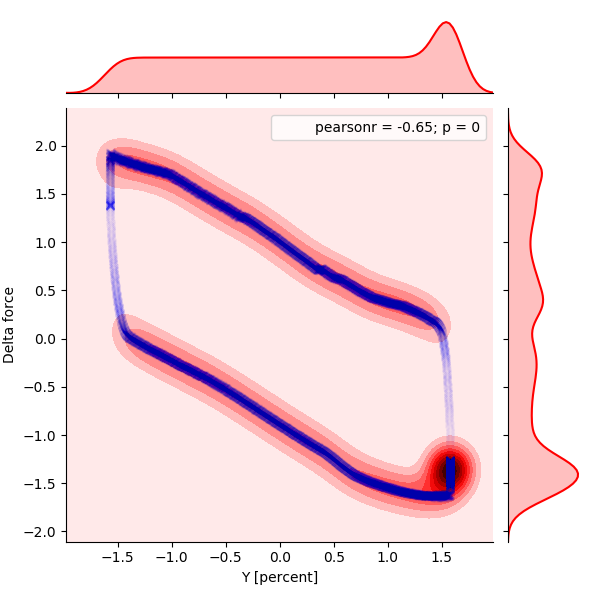
\includegraphics[width=1\linewidth]{figures/data/kdePlot_servoindication_A4.png} 
                \end{minipage}
                  \hfill
                  \begin{minipage}[b]{0.5\linewidth}
                    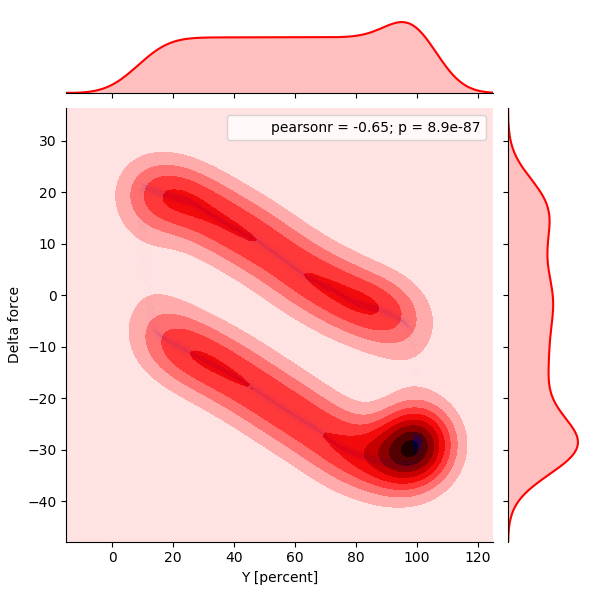
\includegraphics[width=1\linewidth]{figures/data/kdePlot_reduced_Servo_A4.png} 
                \end{minipage} 
                \caption{Kde plots for original servo indication data, and down sampled servo indication data for turbine $4$.}
                \label{fig:kde_servo}
            \end{figure}

        \subsubsection{Scaling}
            The final step of the preprocessing is to scale the each feature. First all samples are mean centered, and they are then scaled to unit variance. The result is shown in Figure \ref{fig:start_up_reduced_4}. Notice that the range of the $X$ and $Y$ axis are now approximately the same. The non linearity seen in Figure \ref{fig:start_up_4} is also removed. The data is now ready for analysis.     
            
            
        
            \begin{figure}[h]
                \centering
                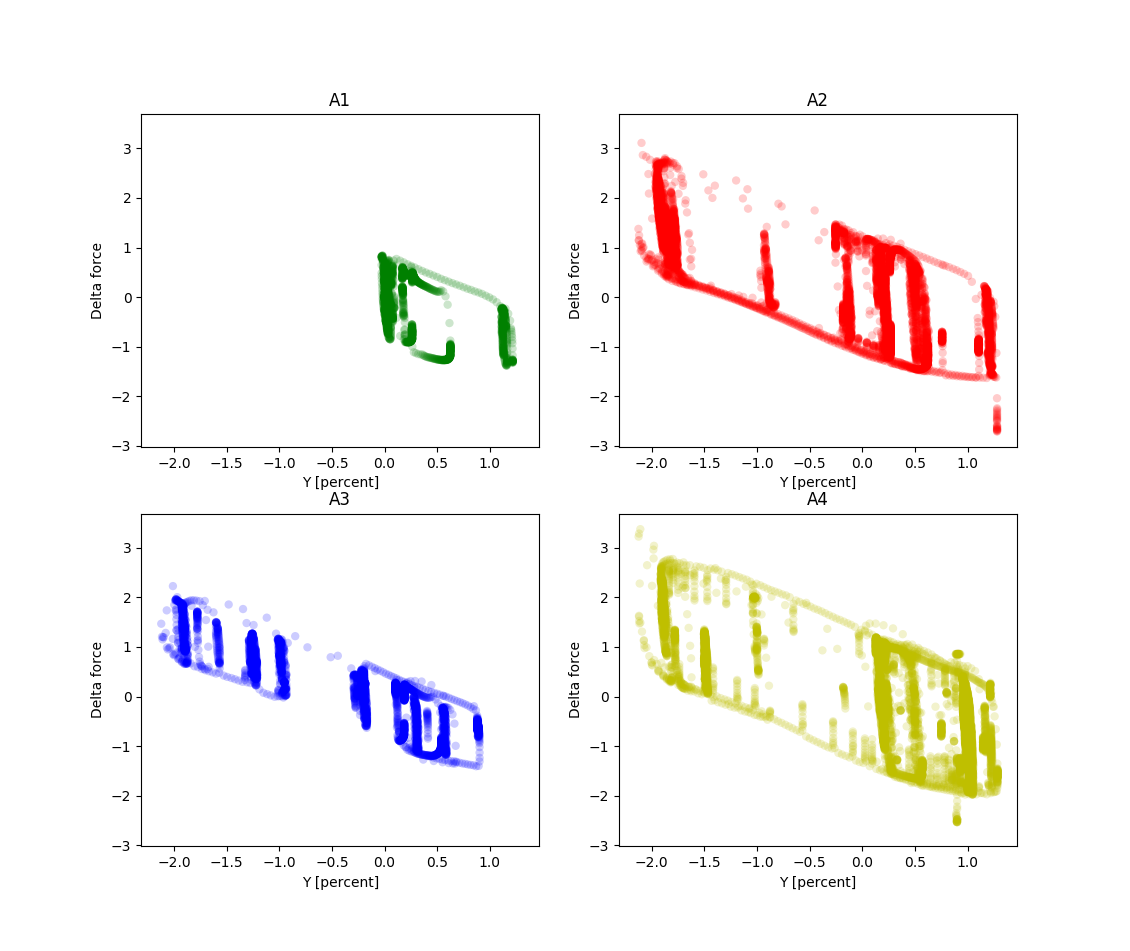
\includegraphics[width = \textwidth]{figures/data/start_up_reduced_4.png}
                \caption{The reduced commissioning data set, here each sample is given an alpha = 0.2, this means that the intensity of the color is high where several samples overlap}
                \label{fig:start_up_reduced_4}
            \end{figure}




\section{Machine learning for classification of guide vane condition}
    The goal is to create a classifier that is able to classify the condition of the guide vanes of a turbine. The problem is attacked from two different angels, using four different methods. The analysis of the servo indication data is presented first, then the analysis for the commissioning data. The first approach uses one class SVM to create a separate classifier for each of the datasets for the four turbines. This is then used to classify new samples as either an inlier or outlier. This means that similar data samples can be classified as inliers for several classifers. 
    
    The tree other methods use multiclass classification. Here the data from the different datasets are given a unique label, and one classifier is created using all four datasets. The classification is performed using logistic regression, support vector machines and neural networks. This means that for the multiclass classification data from all turbines are used simultaneously. Hence a sample can only be predicted to one class as opposed to one class SVM.
    
    All algorithms are evaluated based on the classifiers decision boundaries, and the accuracy of their predictions. The fact that there is only two features in the feature set, makes visual inspection of the decision boundaries possible. Therefore the performance of the different algorithms are mostly evaluated based on the decision boundary plot, and not so much on the prediction accuracy and F1-score. However, if the number of dimensions were to grow, this would not be a sufficient approach.
    
    % It is the performance on the servo indcation sets that are analysed. This means that the classifiers which are created on the start ups set, are used to predict on the servo indication set. This enables one to compare the performance of the two different sets of classifiers. This means that even if the accuracy and f1-score are not of most importance during hyperparameterization, they can be used to evaluate the performance accross the two different sets.   
    
    \subsection{Training and test sets}
        Before the data is fed into the learning algorithms it is split into training and test sets. Since the classifier is not trained on the test set, it can be used to verify how well the classifier performs to new data. This is one of the steps taken to avoid overfitting. The classified data is randomly split into two parts, where $ 25\%$ of the data is in the test set and the rest is in the training set. There is not a clear optimal choice for size of training set, according to \cite{Kohavi1995} somewhere around $1/3$ is common.   
        
        
    \subsection{Servo indication data}
        The first case, is the servo indication data. It is a fair assumption that the performance on these datasets, will most likely be an upper limit for what can be found for the commissioning datasets. The data can be seen in Figure \ref{fig:servo_indication_analysis}. One can see that data from turbine A4 and A2, and A1 and A3 are similar. 
        
        \begin{figure}[]
            \centering
            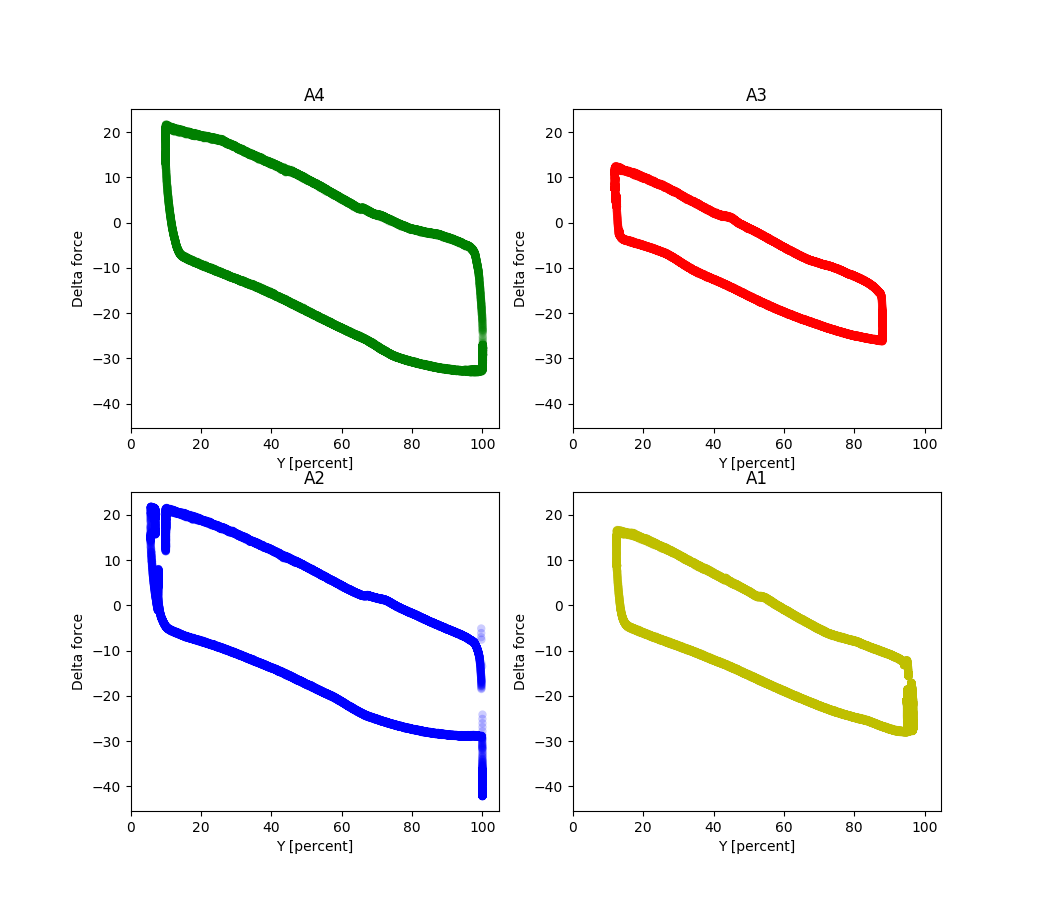
\includegraphics[width=0.8\textwidth]{figures/data/servo_indication_all.png}
            \caption{The servo indication data for the four different turbines}
            \label{fig:servo_indication_analysis}
        \end{figure}
        
        \subsubsection{One class SVM}
            To ensure a good generalization, the optimal hyperparamteters for the one class SVM classifier are found by comparing how well they performed across the different datasets. The classification is performed using Scikit-learn. Optimal hyper parameters are found in a combination between using randomized search and visual inspection of the decision boundary. Figure \ref{fig:hyperparam_oneclass} shows the decision boundary for the A1 dataset for different hyperparameters. Here $\gamma$ is the kernel coefficient and $\nu$ is an upper fractional limit for training errors and a lower fractional limit for support vectors. 
            
            The upper left plot in Figure \ref{fig:hyperparam_oneclass} shows an underfit decision boundary. The shape of the decision boundary is too general, and it does not fit the dataset very closely. Comparing it to Figure \ref{fig:servo_indication_all}, it becomes apparent that it will not yield good classification of the datasets. The chosen support vectors clearly shows that the classifier has only emphasized a small part of the data. The plot in the upper right corner shows an example of overfitting. Here the decision boundary is becoming too complex, and a hole appears in the middle. This means that samples located inside the servo indication boundary, will be classified together with samples on the outside. The lower left plot shows the best general fit, these hyperparameters yielded the best overall result for the four datasets. The decision boundary for optimal hyperparamters for the A1 set is shown in the lower right corner. As can be seen, it fits the dataset more closely than the decision boundary for the generalized parameters. It did however lead to overfitting when used for some of the other sets.
            
            \begin{figure}[]
                \begin{minipage}[b]{0.5\linewidth}
                    \centering
                    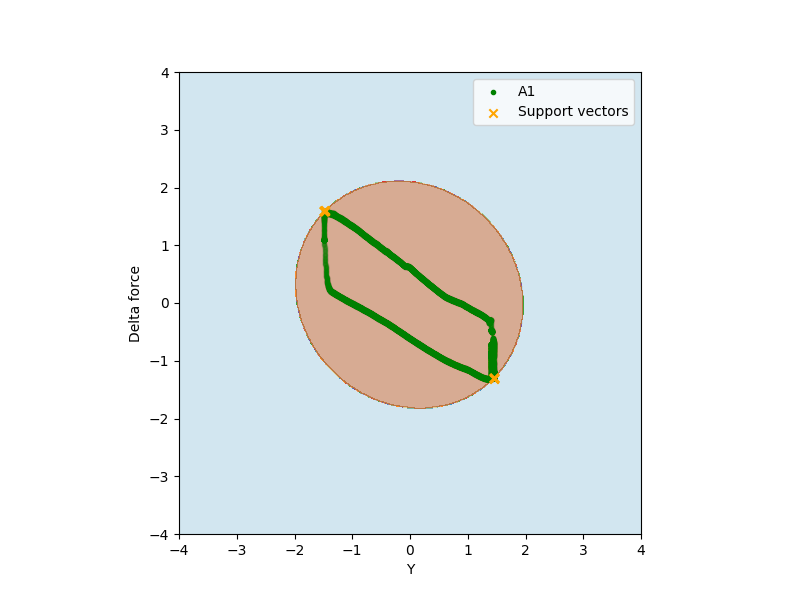
\includegraphics[width = \textwidth]{figures/analysis/oneclass_servo/A1_nu_0001_gamma_002.png}
                    \caption*{Underfit $\gamma = 0.001, \nu = 0.02$, $27$ sup. vectors}
                    % \label{fig:servo_A1_underfit}
                \end{minipage}
                \hfill
                \begin{minipage}[b]{0.5\linewidth}
                    \centering
                    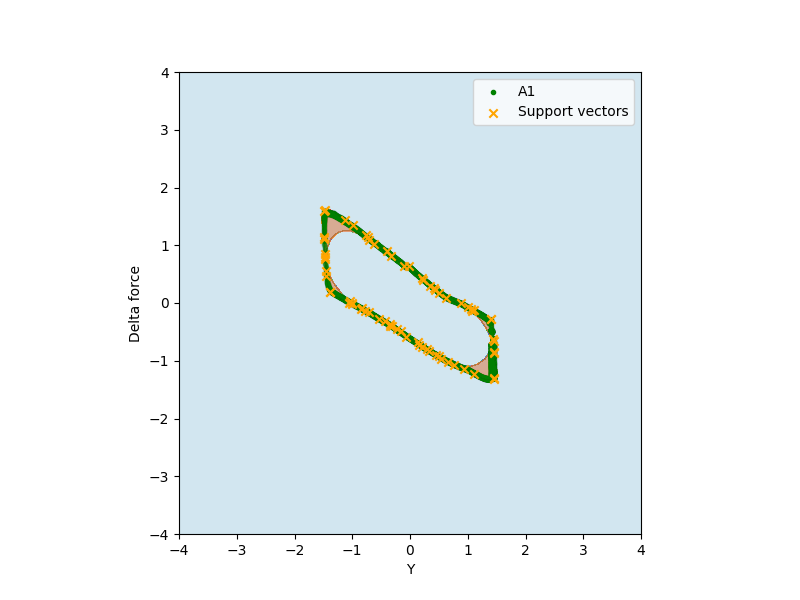
\includegraphics[width = \textwidth]{figures/analysis/oneclass_servo/A1_nu_0001_gamma_8.png}
                    \caption*{Overfit $\gamma = 0.001, \nu = 8$, $69$ sup vectors}
                    % \label{fig:servo_A1_overfit}
                \end{minipage}
                \hfill
                \begin{minipage}[b]{0.5\linewidth}
                    \centering
                    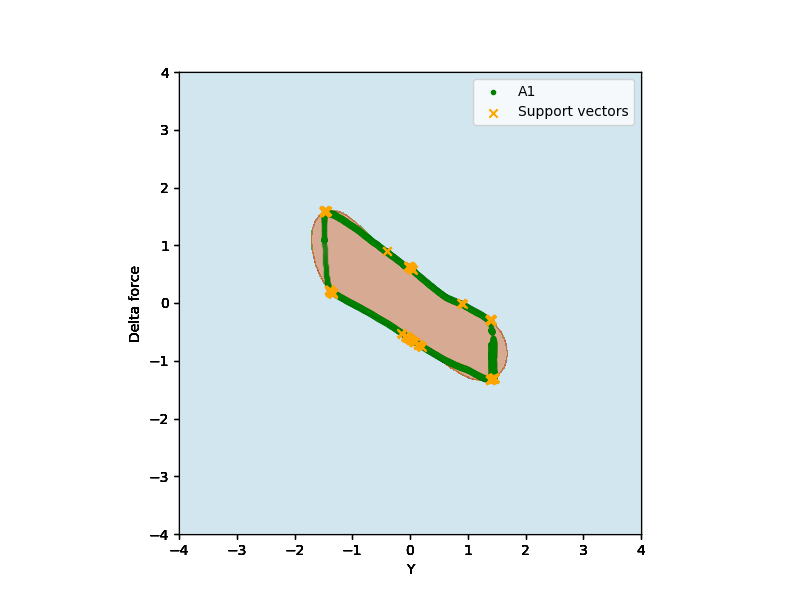
\includegraphics[width = \textwidth]{figures/analysis/oneclass_servo/A1_nu_01_gamma_08.png}
                    \caption*{Best fit for generalization, $\gamma = 0.01, \nu = 0.8$, $265$ sup. vectors}
                    % \label{fig:servo_A1_ok}
                \end{minipage}
                \hfill
                \begin{minipage}[b]{0.5\linewidth}
                    \centering
                    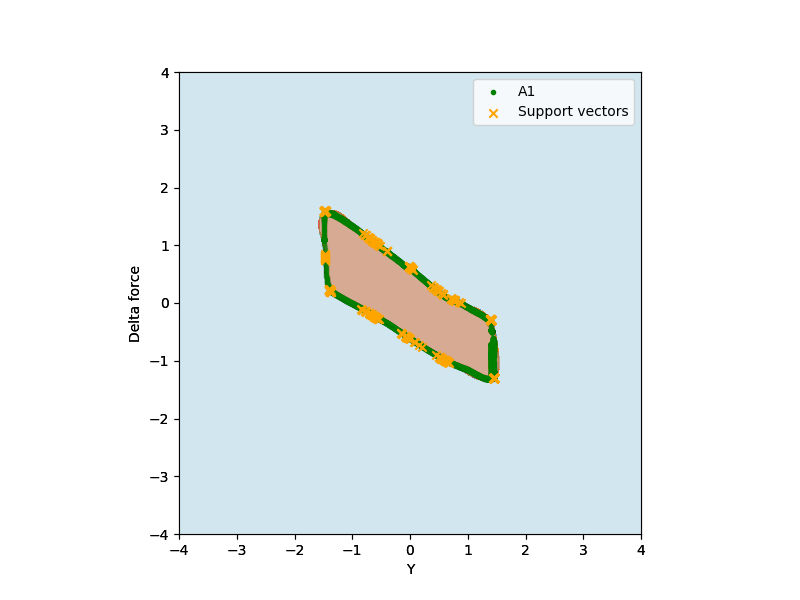
\includegraphics[width = \textwidth]{figures/analysis/oneclass_servo/A1_nu_001_gamma_2.png}
                    \caption*{Best fit for A1 $\gamma = 0.01, \nu = 2$, $268$ sup. vectors}
                    % \label{fig:servo_A1_best}
                \end{minipage}
                \hfill
                \caption{One class svm with different hyperparameters for the A1 dataset. The support vectors used to create the decision boundaries are shown as orange crosses in the plots.}
                \label{fig:hyperparam_oneclass}
            \end{figure}
            
            
            Figure \ref{fig:dec_bound_all_servo} shows the boundaries found for all four datasets using the generalized hyperparameters. The decision boundaries fits the data for all four datasets very well. The worst fit is seen in the upper right corner for turbine A2. The spike seen in the data, creates a blob in the decision boundary. Reducing this more lead to overfitting on the other data sets. Figure \ref{fig:all_classes_servo_oneclass} shows the four decision boundaries plotted on top of each other. Here one can verify that the size of the decision boundary grows as the turbine ages. One can also see that the boundaries are grouped together two and two as mentioned earlier in the section. The plot shows that data that are classified as inliers for the two most worn turbines, and that are close to the boundaries, will be classified as outliers by the classifiers for the two less worn turbines. 
            
            Table \ref{tab:one_class_servo} shows the performance of the different classifiers. The table shows that all classifiers predict its own data as inliers with a very high accuracy. The table also shows prediction accuracy of outliers. Since the turbines are ranged in the following order A3,A1,A2,A4. Only the turbines that shows more wear are used as outliers. Hence the classifier for turbine A4 has no ouliers to predict on. The classifier for turbine A1 shows a very good prediction rate when tested on data from A2 and A4. The classifier for A3 also has a good prediction rate, despite of having samples that overlap with A1, as shown in Figure \ref{fig:servo_indication_all}.  

            
            \begin{figure}[]
                \begin{minipage}[b]{0.5\linewidth}
                    \centering
                    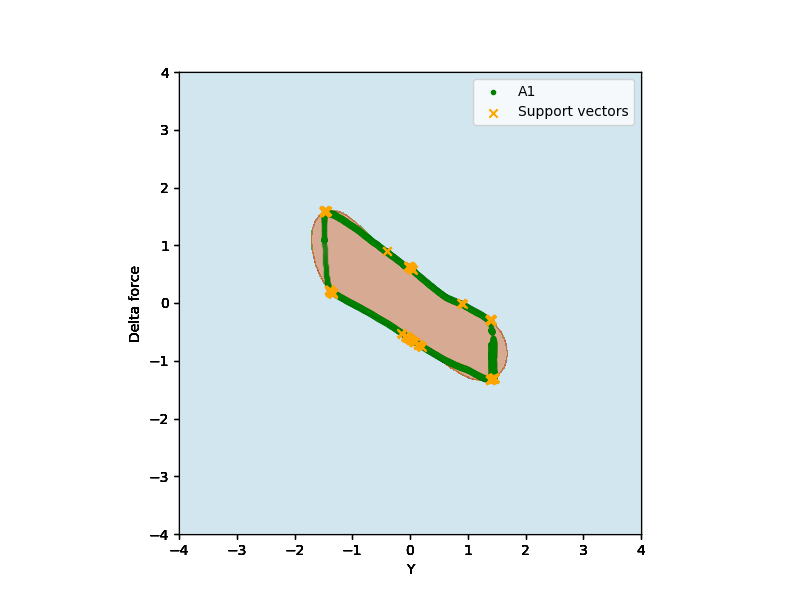
\includegraphics[width = \textwidth]{figures/analysis/oneclass_servo/A1_nu_01_gamma_08.png}
                    \caption*{Decision boundary A1, $\gamma = 0.01, \nu = 0.8$}
                    % \label{fig:servo_A1}
                \end{minipage}
                \hfill
                \begin{minipage}[b]{0.5\linewidth}
                    \centering
                    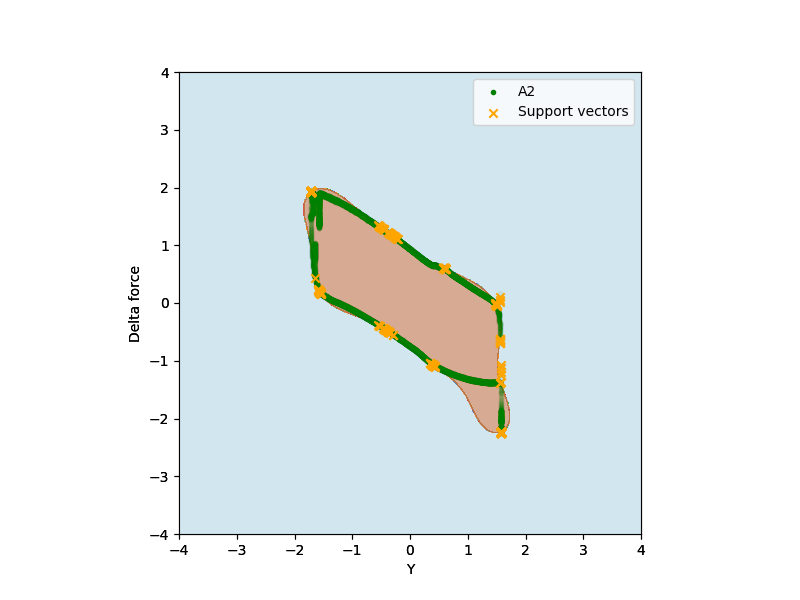
\includegraphics[width = \textwidth]{figures/analysis/oneclass_servo/A2_nu_01_gamma_08.png}
                    \caption*{Decision boundary A2, $\gamma = 0.01, \nu = 0.8$}
                    % \label{fig:servo_A2}
                \end{minipage}
                \hfill
                \begin{minipage}[b]{0.5\linewidth}
                    \centering
                    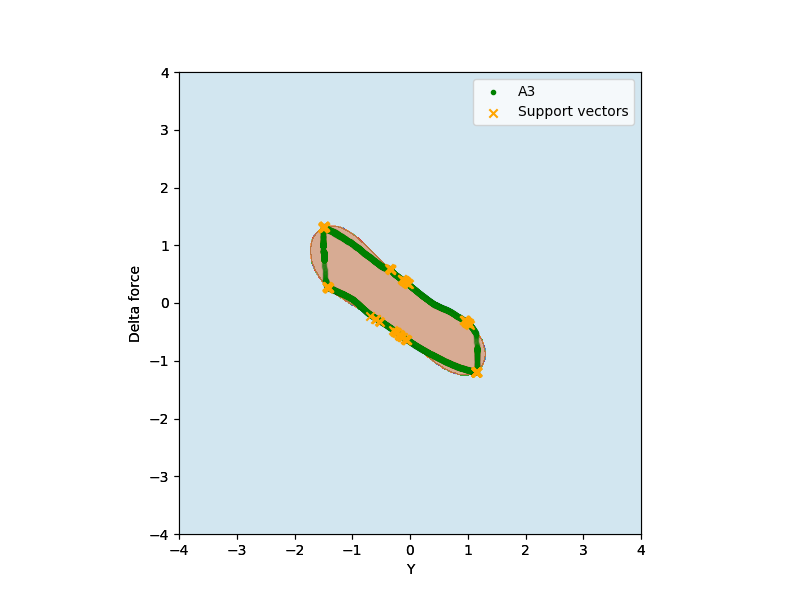
\includegraphics[width = \textwidth]{figures/analysis/oneclass_servo/A3_nu_01_gamma_08.png}
                    \caption*{Decision boundary A3, $\gamma = 0.01, \nu = 0.8$}
                    % \label{fig:servo_A3}
                \end{minipage}
                \hfill
                \begin{minipage}[b]{0.5\linewidth}
                    \centering
                    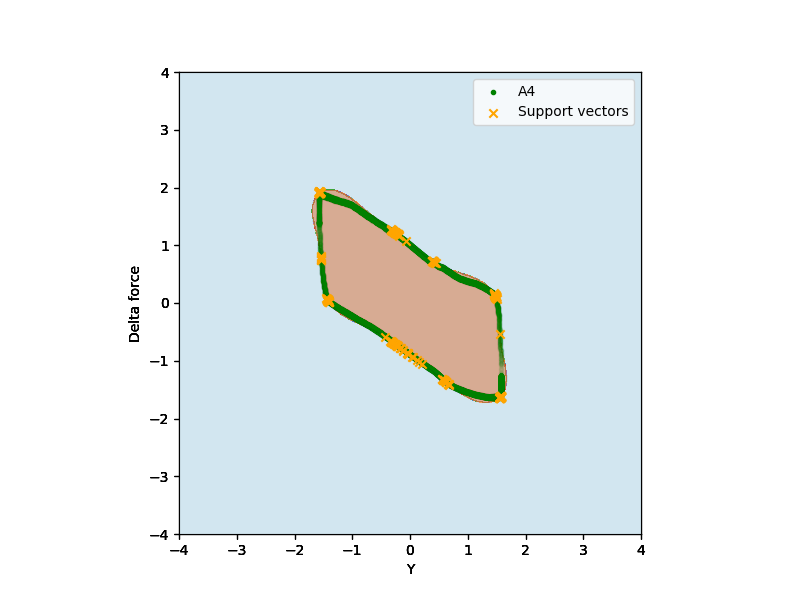
\includegraphics[width = \textwidth]{figures/analysis/oneclass_servo/A4_nu_01_gamma_08.png}
                    \caption*{Decision boundary A4, $\gamma = 0.01, \nu = 0.8$}
                    % \label{fig:servo_A4}
                \end{minipage}
                \hfill
                \caption{Decision boundary for all four servo indication datasets with the best general hyperparameterization. Support vectors are shown in orange.}
                \label{fig:dec_bound_all_servo}
            \end{figure}
            
            
            \begin{figure}[]
                \centering
                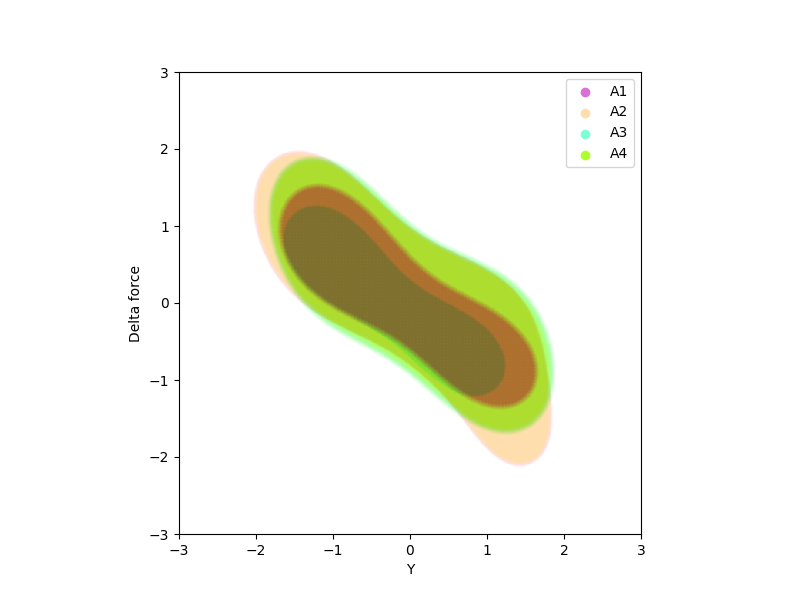
\includegraphics[scale=0.6]{figures/analysis/oneclass_servo/One_Class_SVM_servoIndication.png}
                \caption{All decision boundaries plotted against each other. Due to the overlaying boundaries, the colors does not match the legend}
                \label{fig:all_classes_servo_oneclass}
            \end{figure}
            
            \begin{table}[]
                \centering
                \begin{tabular}{|c|c|c|c|c|c|c|c|c|}
                    \hline
                    Turbine &$\gamma$   & $\nu$     & Acc. train    & Acc. test &Acc. outliers  & Outlier sets  & Sup. vectors  & Samples  \\ \hline
                    A1      & $0.01$    & $0.08$    & $0.990$       & $0.990$   & $0,976$       & A2, A4        &$265$         & $34777$\\ \hline
                    A2      & $0.01$    & $0.08$    & $0.990$       & $0.990$   & $0,626$       & A4            &$274$         & $35411$\\ \hline
                    A3      & $0.01$    & $0.08$    & $0.990$       & $0.990$   & $0,878$       & A1, A2, A4    &$229$         & $29496$\\ \hline
                    A4      & $0.01$    & $0.08$    & $0.990$       & $0.989$   &               &               &$269$         & $35127$\\ \hline
                \end{tabular}
                \caption{Table listing the performance of the optimal one class SVM classifier for the four cases. Note thate $\gamma$ is the kernel coefficient for the rbf kernel, and that $\nu$ is the lower bound on the fraction of support vectors. }
                \label{tab:one_class_servo}
            \end{table}
            
            Figure \ref{fig:learning_curves_A1} shows the learning curves for the classifier for the A1 dataset. The prediciton accuracy starts out low and increases with the training sets. Once above $2000$ samples it converges to $90\%$. Threefold cross validation is used for the training. The standard deviation for the predictions are shown in the colored areas around the lines. 
            
            \begin{figure}[]
                \centering
                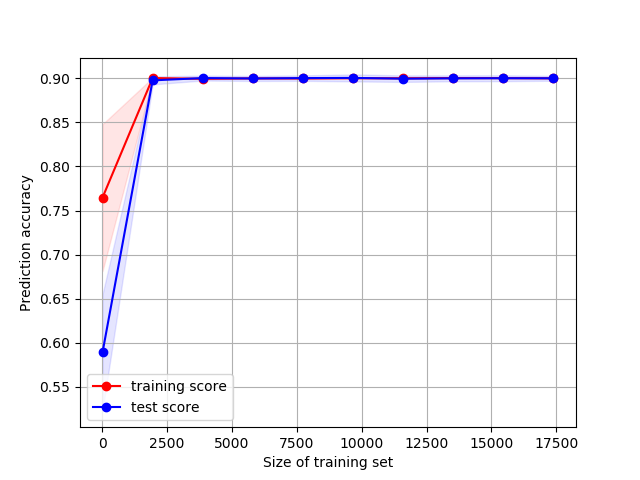
\includegraphics[scale = 0.6]{figures/analysis/oneclass_servo/LearningCurves_A1.png}
                \caption{Learning curve for the A1 classifier, the accuracy of the classifier as a function of the training size.}
                \label{fig:learning_curves_A1}
            \end{figure}
        
        %%%%%%%%%%%%%%%%%%%%%%%%%%%%%%%%%%%%%%%%%%%%%%%%%%%%%%%%%%%%%%%%%%%%%%%%%%%%%%%%%%%%%%%%%%%%%%%%%%%%%%%%%%%%%%%%%%%%%%%%%%%%%%%%%%%%%%%%%%%%%%%%%%%%%%%%%%%%%%%%%%%%%%%%%%%%%%%%
        \clearpage
        \subsubsection{Multiclass SVM}
            
            Figure \ref{fig:svm_optimal_param} shows the decision boundaries created by the optimal classifier according to randomized search for hyperparameters. The four decision boundaries are not as smooth as one could hope for. The classifier is overfitting on the dataset. A good example is the pink blobs appearing outside the space where all the samples are located. This can lead to strange classifications as the data changes. The search for optimal hyperparameters yields the classifier that classifies the most samples to their corresponding class. The fact that this is a two dimensional feature space enables visual verification of the performance of the different classifiers. The poor performance when using a score function, makes this the preferred way to look for the optimal hyperparameterization. However, a drawback with this approach is the time spent searching for the optimal hyperparameters.  For this reason, only the penalization of the error term C, is tuned. Table \ref{tab:svm_servo} shows the performance of the classifier for different values of C. As can be seen the accuracy, individual F1 score and average F1 score is best when C is high. This makes sense since a high C penalizes miss-classification harder. However this came at a cost of the smoothness of the decisioun boundaries, resulting in plots like the one seen in Figure \ref{fig:svm_optimal_param}.  
            
            The decision boundary for the best classifier is shown in Figure \ref{fig:svm_optimal_servo}. Here one can see that the decision boundary for the two inner classes are smoother than what was the case in Figure \ref{fig:svm_optimal_param}. It also becomes apparent how close the data from turbine two and four are. There is only a small area around the two inner classes that are classified as turbine two. The rest is classified as turbine four. Ideally the blobs to the upper left and lower left should not be there, but by increasing C the decision boundaries became less smooth, and by reducing C the classifiers accuracy fell very much. Table \ref{tab:svm_servo} shows that the average accuracy is still above $80\%$ and that the worst class has a F1 score at $75\%$.  
            
            Figure \ref{fig:svm_undefit_servo} shows the decision boundaries with C = $0.001$. This is not a good fit for the data. Here the the error penalization is too low and this leads to a very general decision boundary. The overall accuracy and performance on the individual classes are also poor. Figure \ref{fig:svm_servo_lc} shows the learning curve for the best classifier found. The increase in accuracy flattens out as the number of samples grows beyond 50000. As can be seen the standard deviation from the three fold cross validation is smaller than what was the case for one class SVM.    
            
            \begin{figure}
                \centering
                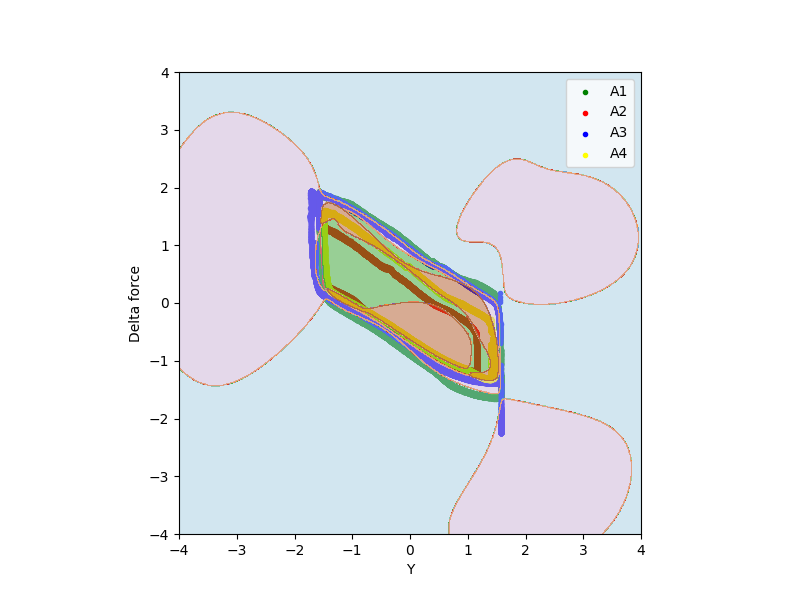
\includegraphics[scale = 0.6]{figures/analysis/svm/SVM-gridOptimal.png}
                \caption{Optimal parameters for SVM found using randomized grid search for optimal hyperparamters, note that due to the transparency the colors of the datasets are not as indicated by the legend.}
                \label{fig:svm_optimal_param}
            \end{figure}
            
            \begin{figure}[]
                \begin{minipage}[b]{0.5\linewidth}
                    \centering
                    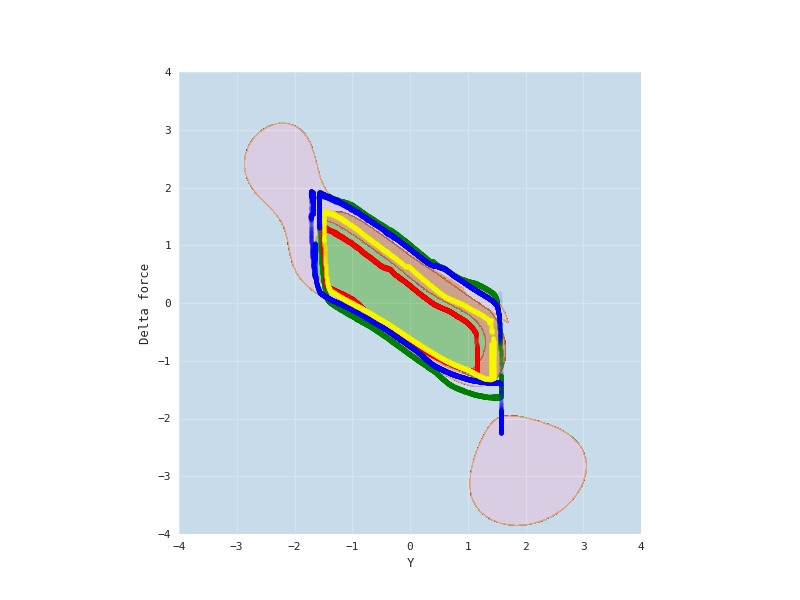
\includegraphics[width = 1.2\textwidth]{figures/analysis/svm/SVM_servo_C01.png}
                    \caption*{Decision boundary C = $0.1$}
                \end{minipage}
                \hfill
                \begin{minipage}[b]{0.5\linewidth}
                    \centering
                    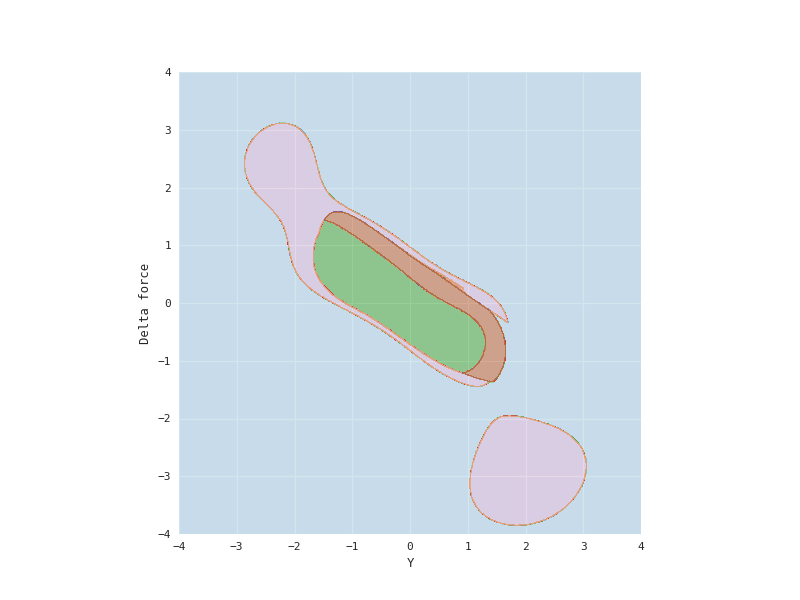
\includegraphics[width = 1.2\textwidth]{figures/analysis/svm/SVM_servo_C01countour.png}
                    \caption*{Decision boundary C = $0.1$}
                \end{minipage}
                \caption{Optimal decision boundary found for SVM.}
                \label{fig:svm_optimal_servo}
            \end{figure}
        
        
            \begin{figure}[]
                \begin{minipage}[b]{0.5\linewidth}
                    \centering
                    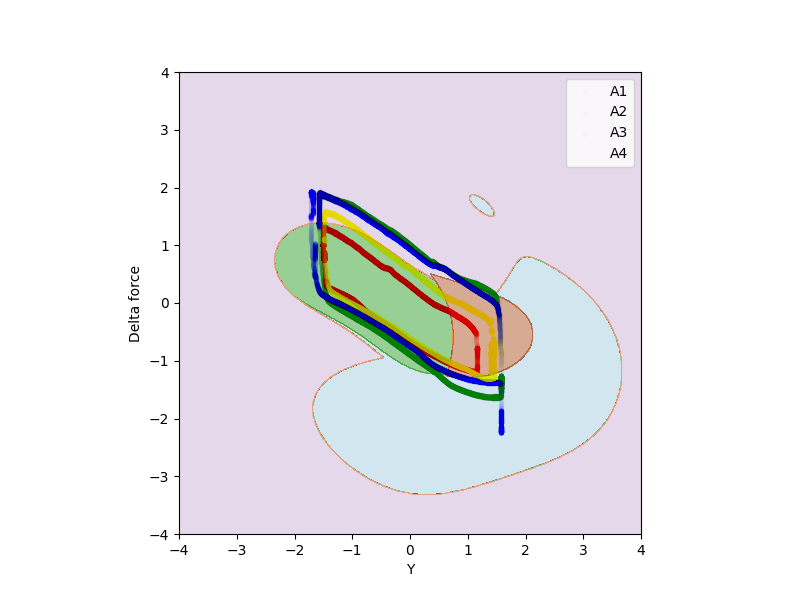
\includegraphics[width = 1.2\textwidth]{figures/analysis/svm/SVM_servo_C0001.png}
                    \caption*{Decision boundary with data, C = $0.001$}
                \end{minipage}
                \hfill
                \begin{minipage}[b]{0.5\linewidth}
                    \centering
                    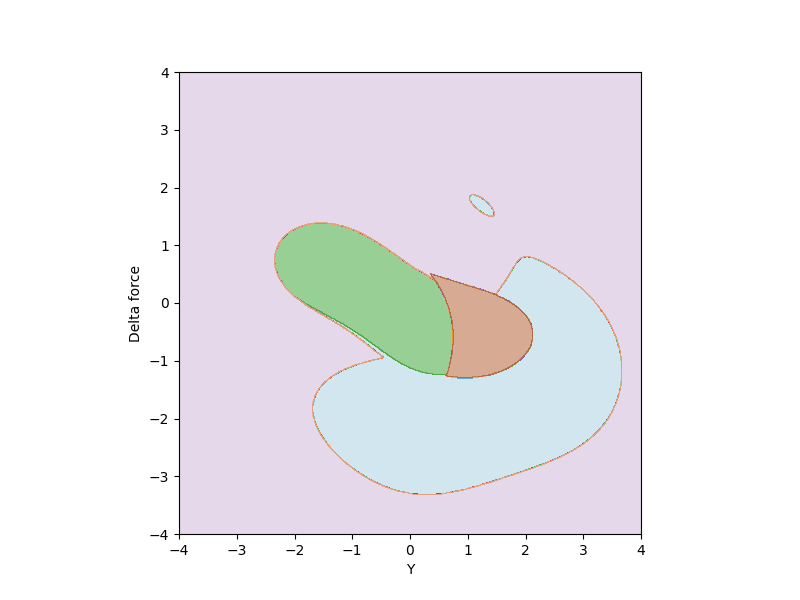
\includegraphics[width = 1.2\textwidth]{figures/analysis/svm/SVM_servo_C0001countour.png}
                    \caption*{Decision boundary  C $= 0.001$}
                \end{minipage}
                \caption{Decision boundary C = 0.001, the decision boundary is too simple, the classifier is underfitted.}
                \label{fig:svm_undefit_servo}
            \end{figure}
        
        
            \begin{table}[]
                \centering
                \begin{tabular}{|c|c|c|c|c|c|c|c|c|c|c|c|c|}
                    \hline
                    C       & $\gamma$  & Kernel    & Accuracy          &F1 A1      &F1 A2      &F1 A3      &F1 A4      & Average F1        &  Sup. vectors  &Samples  \\ \hline
                    $1000$  & Auto      & Rbf       & $0.957$           & $0.951$   & $0.961$   &$0.952$    &$0.966$    & $0.958$           & $12036$           &$101108$\\ \hline
                    $10$    & Auto      & Rbf       & $0.921$           & $0.936$   & $0.901$   &$0.939$    &$0.904$    & $0.919$           & $31762$           &$101108$\\ \hline
                    $2$     & Auto      & Rbf       & $0.876$           & $0.924$   & $0.831$   &$0.932$    &$0.805$    & $0.873$           & $38973$           &$101108$\\ \hline
                    $1$     & Auto      & Rbf       & $0.860$           & $0.922$   & $0.810$   &$0.927$    &$0.765$    & $0.856$           & $42732$           &$101108$\\ \hline
                    $\bm{0.1}$   & \textbf{Auto} &\textbf{Rbf}  &\bm{$0.828$} &\bm{$0.885$} &\bm{$0.795$} &\bm{$0.870$} &\bm{$0.745$}&\bm{$0.824$}&\bm{$67788$}&\bm{$101108$}\\ \hline
                    $0.01$  & Auto      & Rbf       & $0.646$           & $0.592$   & $0.712$   &$0.571$    &$0.704$    & $0.645$           & $94798$           &$101108$\\ \hline
                    % $0.001$ & Auto      & Rbf       & $0.443$           & $0.377$   & $0.519$   &$0.438$    &$0.384$    & $0.430$           & $99244$           & $100$     \\ \hline
                    
                \end{tabular}
                \caption{Table listing the performance of the classifiers for different hyperparameterizations of SVM. C is the regularization coefficient, and gamma is the kernel coefficient, auto = 1/\#features. The best results are shown in bold.}
                \label{tab:svm_servo}
            \end{table}
            
            \begin{figure}
                \centering
                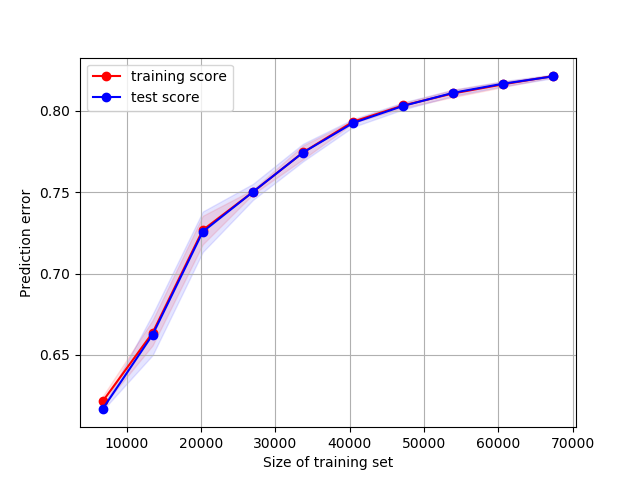
\includegraphics[scale=0.6]{figures/analysis/svm/SVM_servo_C01_LC.png}
                \caption{Learning curve for the best classifier with C $= 0.1$}
                \label{fig:svm_servo_lc}
            \end{figure}
            
            
        %%%%%%%%%%%%%%%%%%%%%%%%%%%%%%%%%%%%%%%%%%%%%%%%%%%%%%%%%%%%%%%%%%%%%%%%%%%%%%%%%%%%%%%%%%%%%%%%%%%%%%%%%%%%%%%%%%%%%%%%%%%%%%%%%%%%%%%%%%%%%%%%%%%%%%%%%%%%%%%%%%%%%%%%%%%%%%%%%    
        \clearpage    
        \subsubsection{Logistic regression}
            The second multiclass analysis is logistic regression. To enable nonlinear decision boundaries, the classification is performed with a range of polynomial extensions. Randomized search was used to get the optimal hyperparameters for each of the polynomial degrees. Figure \ref{fig:poly_ext_servo} shows the decision boundary found for four different polynomial extensions. As could be expected, linear combinations of the original feature space does not yield very good results. The decision boundary can be seen in the upper left plot. Once the polynomial extensions increases above the second degree, the decision boundaries start to take random formations. This is seen in the two bottom plots in Figure \ref{fig:poly_ext_servo}. There are no samples in that space, which means that there is no way for the accuracy and F1-score to penalize the algorithm for this overfitting. In addition the data from the servo indication has some common sample spaces, meaning that the more freedom the classifier is given by having a small regularization term, the better it will adapt to the overlapping part of the dataset. 
            
            Table \ref{tab:logr_reg} show how well the different classifiers performed on the servo indication data. As can be seen the higher the polynomial term, the better the accuracy and F1-scores are. This comes however at the cost of overfitting and a increase in computation time as the feature space grows. At degree nine one can see that the original two dimensional feature space is extended to 55 dimensions. The scores were shown to converge after degree 9, so the analysis was stopped there.
            
            The best decision boundary is at degree two, this is the only nonlinear boundary that does not introduce the random classifications outside the sample space. It is however not a very good classifier, since it only yields $66\%$ accuracy. 
            
            \begin{figure}[]
                \begin{minipage}[b]{0.5\linewidth}
                    \centering
                    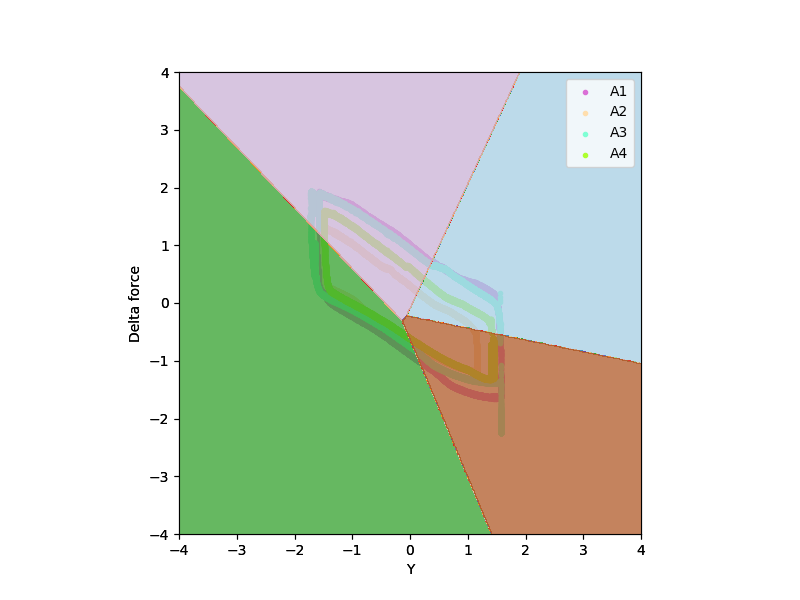
\includegraphics[width = 1\textwidth]{figures/analysis/logistic_regression/Logistic_Regression_degree1.png}
                    \caption*{Decision boundary p.deg $= 1$}
                \end{minipage}
                \hfill
                \begin{minipage}[b]{0.5\linewidth}
                    \centering
                    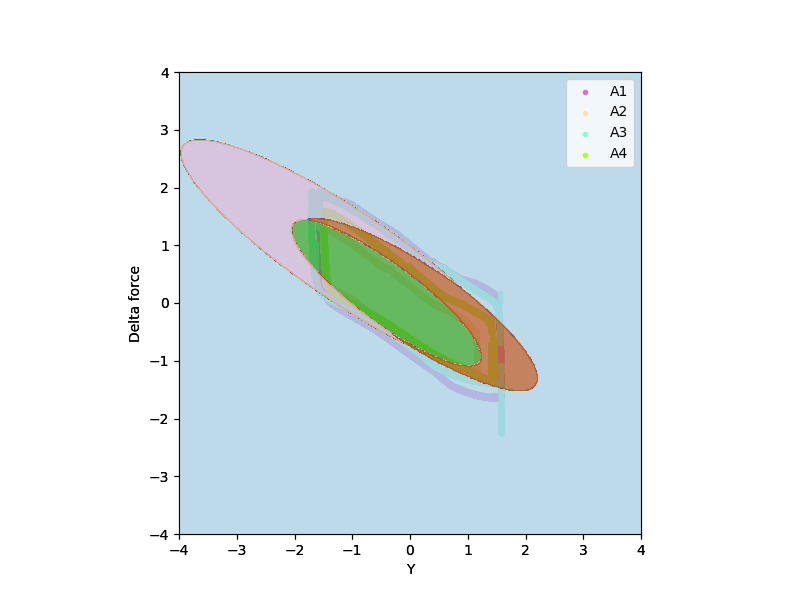
\includegraphics[width = 1\textwidth]{figures/analysis/logistic_regression/Logistic_Regression_degree2.png}
                    \caption*{Decision boundary p.deg $= 2$}
                \end{minipage}
                \hfill
                \begin{minipage}[b]{0.5\linewidth}
                    \centering
                    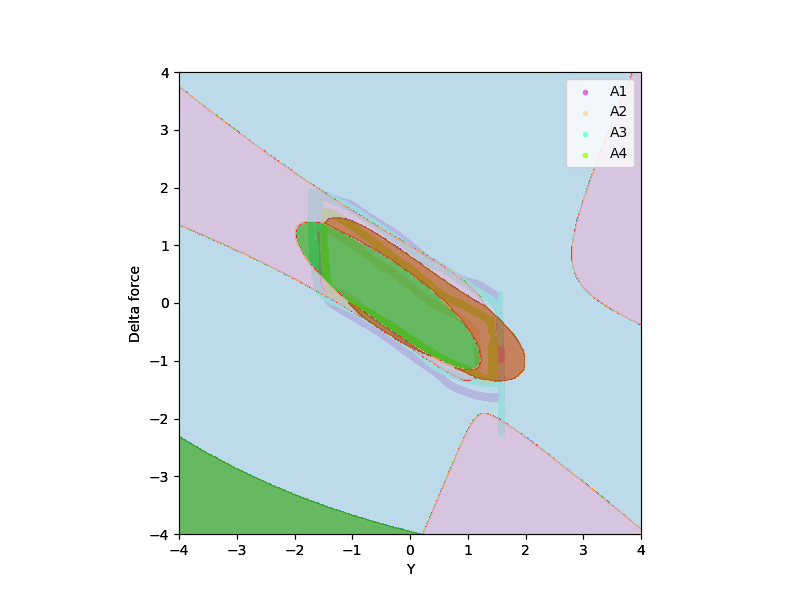
\includegraphics[width = 1\textwidth]{figures/analysis/logistic_regression/Logistic_Regression_degree3.png}
                    \caption*{Decision boundary p.deg $= 3$}
                \end{minipage}
                \hfill
                \begin{minipage}[b]{0.5\linewidth}
                    \centering
                    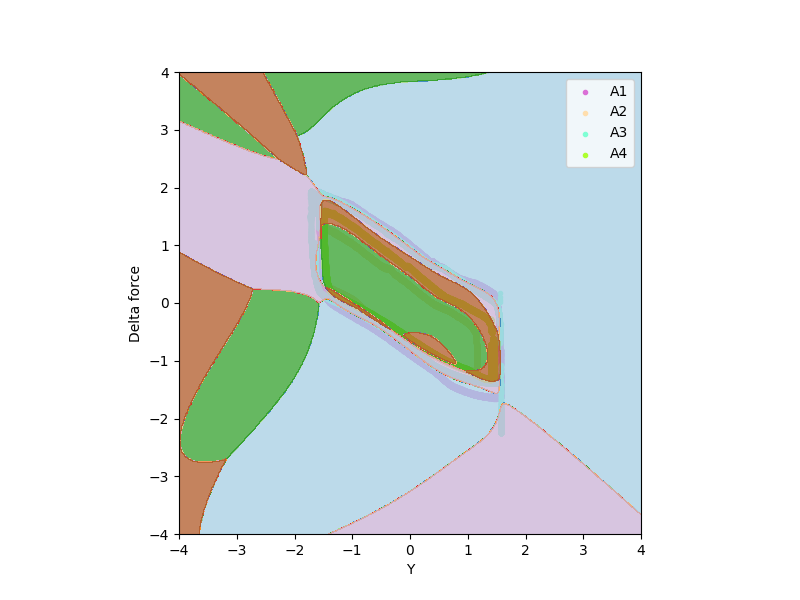
\includegraphics[width = 1\textwidth]{figures/analysis/logistic_regression/Logistic_Regression_degree9.png}
                    \caption*{Decision boundary p.deg $= 9$}
                \end{minipage}
                \hfill
                \caption{Plots showing the decision boundaries for some of the polynomial extensions for the LR classifers. The contours of the servo indication data are seen transparent on top of the decision boundary.}
                \label{fig:poly_ext_servo}
            \end{figure}
            
            
            \begin{figure}[]
                \centering
                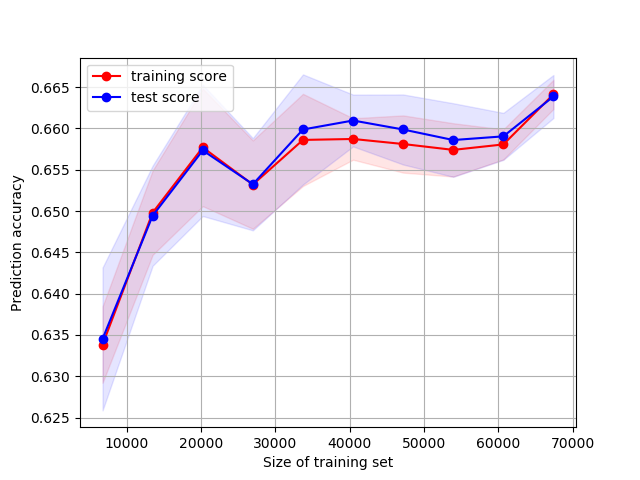
\includegraphics[scale = 0.6]{figures/analysis/logistic_regression/LearningCurves_degree2.png}
                \caption{Learning curve for polynomial extension to the second degree. }
                \label{fig:log_reg_lc}
            \end{figure}
            
            Figure \ref{fig:log_reg_lc} shows the learning curves for the classifier trained on the second degree polynomial extension feature set. The accuracy increases as more training examples are added. The colored area around the bars shows the standard deviation $\sigma$ for the accuarcy. As can be seen $\sigma$ is reduced as the number of training samples grows. Three fold crossvalidation is used, and the standard deviation $\sigma$ is calcualted from this.  
            
            
            \begin{table}[]
                \centering
                \begin{tabular}{|c|c|c|c|c|c|c|c|c|c|c|c|}
                    \hline
                    Poly. deg.  & C     & Accuracy  &F1 A1      &F1 A2      &F1 A3      &F1 A4      & Average F1    &  Features  \\ \hline
                     $1$        & $1$   & $0.303$    & $0.195$    & $0.320$    & $0.332$    & $0.342$    & $0.285$       & $3$\\ \hline
                     $\bm{2}$        & $\bm{1}$   & $\bm{0.662}$    & $\bm{0.709}$    & $\bm{0.732}$    & $\bm{0.584}$    & $\bm{0.617}$    & $\bm{0.661}$        & $\bm{6}$\\ \hline
                     $3$        & $1$   & $0.670$    & $0.709$    & $0.770$    & $0.544$    & $0.637$    & $0.665$        & $10$\\ \hline
                     $4$        & $1$   & $0.794$    & $0.844$    & $0.745$    & $0.835$    & $0.744$    & $0.792$        & $15$\\ \hline
                     $5$        & $1$   & $0.831$    & $0.900$    & $0.767$    & $0.885$    & $0.762$    & $0.829$        & $21$\\ \hline
                     $6$        & $1$   & $0.872$    & $0.920$    & $0.816$    & $0.919$    & $0.826$    & $0.870$        & $28$\\ \hline
                     $7$        & $1$   & $0.881$    & $0.927$    & $0.822$    & $0.930$    & $0.835$    & $0.879$        & $36$\\ \hline
                     $8$        & $1$   & $0.902$    & $0.936$    & $0.860$    & $0.940$    & $0.865$    & $0.900$        & $45$\\ \hline
                     $9$        & $1$   & $0.914$    & $0.946$    & $0.878$    & $0.946$    & $0.881$    & $0.913$        & $55$\\ \hline
                \end{tabular}
                \caption{Table listing the performance of the classifiers for the different polynomial extensions. The C parameter is the regularization term. The best result is shown in bold.}
                \label{tab:logr_reg}
            \end{table}
        
        %%%%%%%%%%%%%%%%%%%%%%%%%%%%%%%%%%%%%%%%%%%%%%%%%%%%%%%%%%%%%%%%%%%%%%%%%%%%%%%%%%%%%%%%%%%%%%%%%%%%%%%%%%%%%%%%%%%%%%%%%%%%%%%%%%%%%%%%%%%%%%%%%%%%%%%%%%%%%%%%%%%%%%%%%%%%%%%%%%%%%%%%%%%%%%%%%%%%%%%
        \clearpage
        \subsubsection{Neural network}
            As the scoring function were shown not to be a good fit for evaluation of the best hyperparameters for the different algorithms, the NN analysis was also performed by visual inspection of the decision boundary. This is however much more complex for a NN then for SVM and LR. The possible combinations of hyperparameters becomes very large for a NN. First the height and depth of the network must be decided. Already there the number of possible sensible options grows beyond what one can manually analyze in reasonable time. The type of solver, weight initialization, batch size and number of epochs also will yield different results. Optimizing all these hyperparameters is too time consuming, so only a selection of height, depth, epochs and batch sizes are tuned. This means it is not possible to say if the results achieved are optimal. Nadam is chosen as optimizer for all the tests, which is an improvement of the familiar Adam algorithm \cite{Dozat}. 
            
            One important factor that was found during the NN anlysis, was that changing the number used as seed for the generation of random numbers in python, had a big impact on the decision boundary the classifier produced. The impact was largest on the outside of the sample space. This makes sense, since the lack of samples makes it impossible for the algorithm to analyze how the weight coefficients change the decision boundary outside the sample space. Optimizing a neural network is in many cases not a convex optimization problem \cite{Hastie}. This means that changing the initial value for the weight coefficients can lead to the algorithm converging at a new local minima, producing very different results.
            
            Figure \ref{fig:nn_servo_best_fit} shows the decision boundary for the best classifier found by visual inspection. It fits the training data well, and does not overfit any of the inner classes. As can be seen in row  three in Table \ref{tab:nn_servo}, the prediction accuracy for this classifier is $92\%$. All the indiviudal F1-scores are also above $90\%$ which indicates that it is performing very well on all classes. It is outperforming both multiclass SVM and LR. 
            
            Figure \ref{fig:nn_servo_overfit} shows the decision boundary for a classifier with ten neurons in each hidden layer. The added height increases the complexity of the NN, and results in an overfit decision boundary. If a really worn down turbine was classified using this classifier, it is a risk that it will be classified with the same degree of wear as turbine A2, and not as turbine A4 which should be the case. Still, row seven in the table shows that it by the scoring functions, are performing better than the classifier with the best decision boundary.  
            
            Figure \ref{fig:nn_servo_underfit} shows the decision boundary for a classifier with only 3 neurons in each hidden layer. This is NN is clearly underfitting on the data, predicting that almost all samples belongs to the same class. The poor perfomance is also easily verified in row one of Table \ref{tab:nn_servo}. Figure \ref{fig:model_accuracy_nn} shows the prediction accuracy of the best classifier as a function of increasing number of epochs. The figure shows that after $200$ epochs the classifier is no longer improving its predictions.
            
            
            \begin{table}[]
                \centering
                \begin{tabular}{|c|c|c|c|c|c|c|c|c|c|c|c|c|}
                    \hline
                Row  &Epochs. & Batch size    & Accuracy  &F1 A1      &F1 A2      &F1 A3      &F1 A4      & Average F1    &  Depth    & Height  \\ \hline
                1&     $500$  & $10000$       & $0.260$   & $0.0$     & $0.0$     & $0.414$   & $0.0$     & $0.104$       & $3$       & $3$     \\ \hline
                2&     $500$  & $500$         & $0.94$    & $0.952$   & $0.924$   & $0.954$   & $0.936$   & $0.942$       & $3$       & $5$     \\ \hline
                    %  $500$  & $500$         & $0.962$   & $0.956$   & $0.965$   & $0.956$   & $0.970$   & $0.962$       & $34777$   &\\ \hline
                    %  $150$  & $1000$        & $0.934$   & $0.942$   & $0.915$   & $0.948$   & $0.932$   & $0.934$       & $3$       & $5$     \\ \hline
                3&     $\bm{500}$  & $\bm{10000}$   & $\bm{0.923}$  & $\bm{0.913}$  & $\bm{0.920}$   & $\textbf{0.922}$   & $\bm{0.937}$   & $\bm{0.923}$ & $\bm3$       & $\bm5$     \\ \hline
                4&     $500$  & $20000$       & $0.895$   & $0.908$   & $0.868$   & $0.915$   & $0.887$   & $0.895$       & $3$       & $5$     \\ \hline
                5&     $750$  & $40000$       & $0.896$   & $0.863$   & $0.863$   & $0.915$   & $0.888$   & $0.895$       & $3$       & $5$     \\ \hline
                6&     $750$  & $40000$       & $0.896$   & $0.863$   & $0.863$   & $0.915$   & $0.888$   & $0.895$       & $3$       & $5$     \\ \hline
                7&     $500$  & $10000$       & $0.938$   & $0.916$   & $0.951$   & $0.923$   & $0.963$   & $0.938$       & $3$       & $10$     \\ \hline
                8&     $1000$ & $40000$       & $0.934$   & $0.916$   & $0.942$   & $0.925$   & $0.954$   & $0.934$       & $3$       & $10$     \\ \hline
                9&     $1000$ & $80000$       & $0.911$   & $0.911$   & $0.901$   & $0.914$   & $0.917$   & $0.911$       & $3$       & $10$     \\ \hline
                    %  $250$  & $80000$       & $0.641$   & $0.720$   & $0.630$   & $0.547$   & $0.635$   & $0.633$       & $3$       & $5$     \\ \hline
                    %  $150$  & $10000$       & $0.912$   & $0.912$   & $0.910$   & $0.912$   & $0.913$   & $0.912$       & $3$       & $10$     \\ \hline
                    %  $150$  & $40000$       & $0.800$   & $0.860$   & $0.786$   & $0.830$   & $0.711$   & $0.800$       & $3$       & $10$     \\ \hline
                    %  $250$  & $80000$       & $0.780$   & $0.837$   & $0.780$   & $0.809$   & $0.692$   & $0.780$       & $3$       & $10$     \\ \hline
                     
                \end{tabular}
                \caption{Table listing the performance of the NN classifiers. The best results are shown in bold.}
                \label{tab:nn_servo}
            \end{table}
            
            \begin{figure}[]
                \begin{minipage}[b]{0.5\linewidth}
                    \centering
                    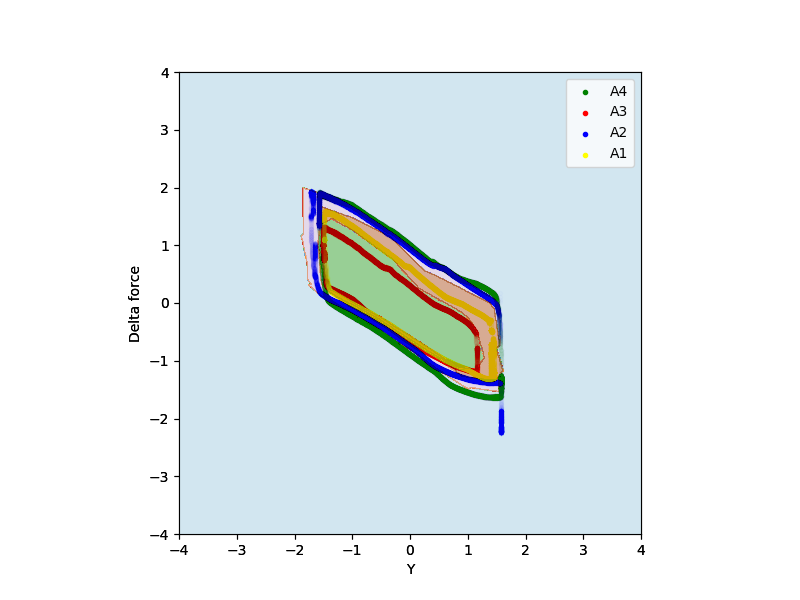
\includegraphics[width = 1\textwidth]{figures/analysis/nn/neural_net_h5_d3_e500_b10000.png}
                    \caption*{Decision boundary with servo indication data}
                \end{minipage}
                \hfill
                \begin{minipage}[b]{0.5\linewidth}
                    \centering
                    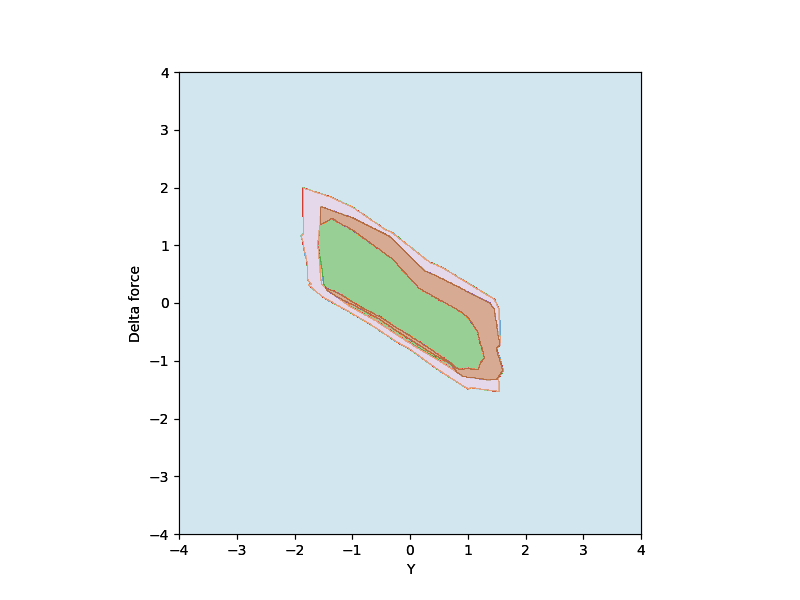
\includegraphics[width = 1\textwidth]{figures/analysis/nn/neural_net_h5_d3_e500_b10000countour.png}
                    \caption*{Decision boundary}
                \end{minipage}
                \caption{NN analysis with depth $= 3$, height $=5$, batch size $=10000$ and epochs $=500$}
                \label{fig:nn_servo_best_fit}
                
            \end{figure}
            
            \begin{figure}[]
                \begin{minipage}[b]{0.5\linewidth}
                    \centering
                    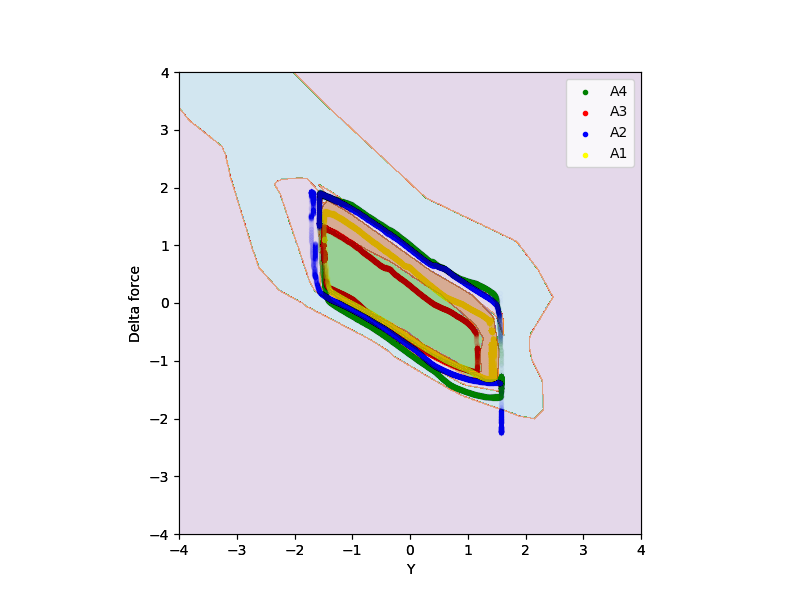
\includegraphics[width = 1\textwidth]{figures/analysis/nn/neural_net_h10_d3_e500_b10000.png}
                    \caption*{Decision boundary with servo indication data}
                \end{minipage}
                \hfill
                \begin{minipage}[b]{0.5\linewidth}
                    \centering
                    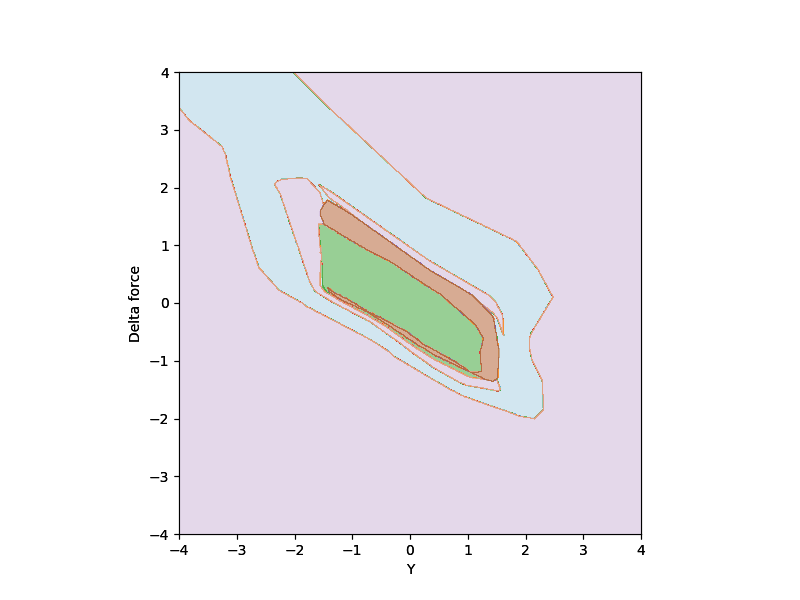
\includegraphics[width = 1\textwidth]{figures/analysis/nn/neural_net_h10_d3_e500_b10000countour.png}
                    \caption*{Decision boundary}
                \end{minipage}
                \caption{NN analysis with depth $= 3$, height $=10$, batch size $=10000$ and epochs $=500$ }
                \label{fig:nn_servo_overfit}
            \end{figure}
            
            \begin{figure}[]
                \begin{minipage}[b]{0.5\linewidth}
                    \centering
                    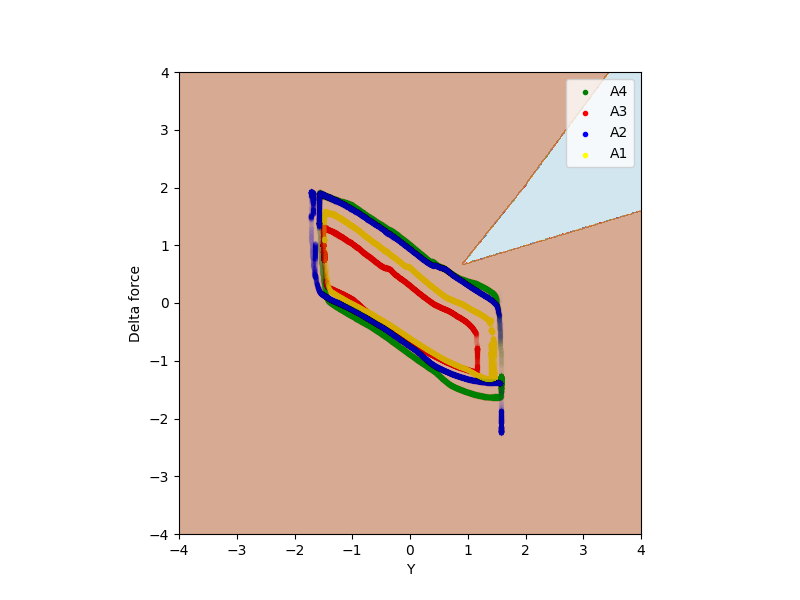
\includegraphics[width = 1\textwidth]{figures/analysis/nn/neural_net_h3_d3_e500_b10000.png}
                    \caption*{Decision boundary with data}
                \end{minipage}
                \hfill
                \begin{minipage}[b]{0.5\linewidth}
                    \centering
                    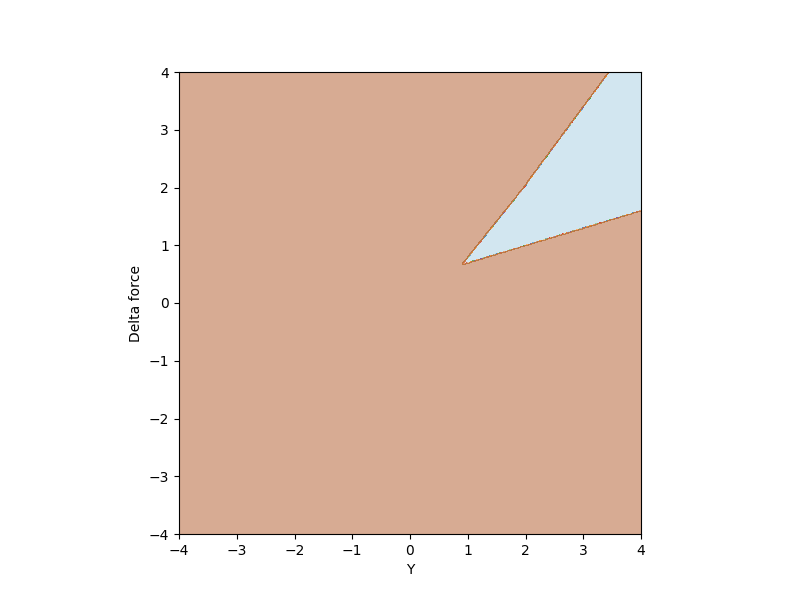
\includegraphics[width = 1\textwidth]{figures/analysis/nn/neural_net_h3_d3_e500_b10000countour.png}
                    \caption*{Decision boundary}
                \end{minipage}
                \caption{NN analysis with depth $= 3$, height $=3$, batch size $=10000$ and epochs $=500$}
                \label{fig:nn_servo_underfit}
            \end{figure}
        
            \begin{figure}
                \centering
                \includegraphics[scale = 0.6]{figures/analysis/nn/model_accuarcy_NN_500_10000_h5_d3.pdf}
                \caption{Accuracy as a function of number of epochs for the best NN classifier}
                \label{fig:model_accuracy_nn}
            \end{figure}
        
        \clearpage
    \subsection{Commissioning dataset}
        This part of the analysis seeks to find if it is possible to extract the same information about the condition of the guide vanes in the turbines from the commissioning dataset as from the servo indication dataset. The downsampled commissioning datasets shown in Figure \ref{fig:start_up_reduced_4} are used. It was made an attempt to perform the analysis with the full datasets, but this lead to a large increase in computation time. This was most apparent for the SVM anlysis. This is supported by the following quote from \cite{Joachims1998}, "In particular, for large learning tasks with many training examples, off the shelf optimization techniques for general quadratic programs quickly become intractable in their memory and time requirements"
        \subsubsection{One class SVM}
            Figure \ref{fig:one_svm_commissioning} shows the once class SVM decision boundaries found for the commissioning data sets, for the best hyperparameters. The upper left plot shows the commissioning data for turbine A1. Since the samples for turbine A1 does not span the full range of $Y$, the resulting decision boundary becomes narrower than for the servo indication case. The three other cases are seen in the rest of the plots. The shape of the boundaries are very similar to the ones for the servo indication case. Notice that none of the feature vectors located inside the decision boundary are used as support vectors. This indicates that the hyperparameterization used enables the algorithm to extract the valueable information from the data. A lot of the data in the commissioning dataset are located inside the outer boundary, hence using them as support vectors will only lead to overfitting.
            
            The servo indication datasets are plotted along with the classifiers decision boundaries for the commissioning datasets in Figure \ref{fig:one_svm_servo}. As expected, the boundary for the A1 classifier is not a very good match with the servo indication data. The three other boundaries are far better, but as can be seen in the figure they are all a little too steep compared to the servo indication data. Table \ref{tab:one_class_startup} shows that the prediction rate on the training data is almost identical to the rate seen for the servo indication. Note that the hyperparameters are changed, and that $\gamma = 0.2$ and $\nu = 0.1$. Table \ref{tab:one_svm_outlier} shows how well the classifiers from the commissioning data predicts inliers and outliers on both the servo indication and the commissioning data. As expected the performance on turbine A1 is poor for the servo indication. The three other classifiers do quite well, averaging around $80\%$ correct predictions of inliers on the servo indication. A more interesting study is how well the classifiers predict outliers for both datasets. For the servo indication, the classifier for turbine A1 is not a good example, due to its small boundary. Since the data for A2 and A4 are so similar, the only classifier that is discussed is the one for turbine A3. It predicts $74\%$ of the data from the three other datasets as outliers. This is not too bad when compared to the $88\%$ predicted by the servo indication classifier for turbine A3. This shows that the decision boundaries for the commissioning dataset is replicating the one for the servo indication. This hypothesis is further strengthen when looking at Figure \ref{fig:all_classes_startup_oneclass} and Figure \ref{fig:one_svm_servo}
            
            Returning to the commissioning dataset, one can see that the classifier for turbine A3 has a $53\%$ prediction accuracy for outliers from the commissioning set. Looking at Figure \ref{fig:one_svm_commissioning} one can see that the three datasets used as outliers, A1,A2 and A4, all have lot of samples located in the middle of the decision boundary. Hence it makes sense that the outlier prediction rate is lower than for the servo indication. 
            
            \begin{figure}[]
                \begin{minipage}[b]{0.5\linewidth}
                    \centering
                    \includegraphics[width = \textwidth]{figures/analysis/oneclass_servo/SVM_one_class_A1_startup_nu_01_gamma_02.png}
                    \caption*{Decision boundary A1, $\gamma = 0.1, \nu = 0.2$}
                    % \label{fig:servo_A1}
                \end{minipage}
                \hfill
                \begin{minipage}[b]{0.5\linewidth}
                    \centering
                    \includegraphics[width = \textwidth]{figures/analysis/oneclass_servo/SVM_one_class_A2_startup_nu_01_gamma_02.png}
                    \caption*{Decision boundary A2, $\gamma = 0.1, \nu = 0.2$}
                    % \label{fig:servo_A2}
                \end{minipage}
                \hfill
                \begin{minipage}[b]{0.5\linewidth}
                    \centering
                    \includegraphics[width = \textwidth]{figures/analysis/oneclass_servo/SVM_one_class_A3_startup_nu_01_gamma_02.png}
                    \caption*{Decision boundary A3, $\gamma = 0.1, \nu = 0.2$}
                    % \label{fig:servo_A3}
                \end{minipage}
                \hfill
                \begin{minipage}[b]{0.5\linewidth}
                    \centering
                    \includegraphics[width = \textwidth]{figures/analysis/oneclass_servo/SVM_one_class_A4_startup_nu_01_gamma_02.png}
                    \caption*{Decision boundary A4, $\gamma = 0.1, \nu = 0.2$}
                    % \label{fig:servo_A4}
                \end{minipage}
                \hfill
                \caption{Decision boundaries one class SVM for the commissioning data using, the best general hyperparameterization. Support vectors shown as orange crosses.}
                \label{fig:one_svm_commissioning}
            \end{figure}
            
            \begin{figure}[]
                \begin{minipage}[b]{0.5\linewidth}
                    \centering
                    \includegraphics[width = \textwidth]{figures/analysis/one_class_startup/SVM_OC_startup_no_servo_g02_nu01_A1.png}
                    \caption*{Decision boundary A1, $\gamma = 0.1, \nu = 0.2$}
                    % \label{fig:servo_A1}
                \end{minipage}
                \hfill
                \begin{minipage}[b]{0.5\linewidth}
                    \centering
                    \includegraphics[width = \textwidth]{figures/analysis/one_class_startup/SVM_OC_startup_no_servo_g02_nu01_A2.png}
                    \caption*{Decision boundary A2, $\gamma = 0.1, \nu = 0.2$}
                    % \label{fig:servo_A2}
                \end{minipage}
                \hfill
                \begin{minipage}[b]{0.5\linewidth}
                    \centering
                    \includegraphics[width = \textwidth]{figures/analysis/one_class_startup/SVM_OC_startup_no_servo_g02_nu01_A3.png}
                    \caption*{Decision boundary A3, $\gamma = 0.1, \nu = 0.2$}
                    % \label{fig:servo_A3}
                \end{minipage}
                \hfill
                \begin{minipage}[b]{0.5\linewidth}
                    \centering
                    \includegraphics[width = \textwidth]{figures/analysis/one_class_startup/SVM_OC_startup_no_servo_g02_nu01_A4.png}
                    \caption*{Decision boundary A4, $\gamma = 0.1, \nu = 0.2$}
                    % \label{fig:servo_A4}
                \end{minipage}
                \hfill
                \caption{Decision boundaries one class SVM commissioning classifiers plotted with the servo indication data.}
                \label{fig:one_svm_servo}
            \end{figure}
            
            
            Figure \ref{fig:all_classes_startup_oneclass} shows the decision boundaries for the four turbines plotted in the same plot. The boundary for A2 and A4 are very similar, almost having the same shape. The boundary for A1 is what makes this very different from the servo indication set. The lack of data makes the classifier unable to recreate a similar shape as found for the servo indication.
            
            
            \begin{figure}[]
                \centering
                \includegraphics[scale=0.6]{figures/analysis/oneclass_servo/All_classes_One_SVM_startup.png}
                \caption{All decision boundaries plotted against each other. Due to the overlaying boundaries, the colors are not as they should}
                \label{fig:all_classes_startup_oneclass}
            \end{figure}
            
            
            \begin{table}[]
                \centering
                \begin{tabular}{|c|c|c|c|c|c|c|c|c|c|}
                    \hline
                    Turbine &$\gamma$   & $\nu$     & Acc. train    & Acc. test & Sup. vectors  & Samples  \\ \hline
                    A1      & $0.2$    & $0.1$    & $0.900$       & $0.923$   &$169$         & $1674$\\ \hline
                    A2      & $0.2$    & $0.1$    & $0.900$       & $0.909$   &$596$         & $5931$\\ \hline
                    A3      & $0.2$    & $0.1$    & $0.900$       & $0.897$   &$306$         & $3047$\\ \hline
                    A4      & $0.2$    & $0.1$    & $0.900$       & $0.909$   &$809$         & $8067$\\ \hline
                \end{tabular}
                \caption{Table listing the performance of the optimal one class SVM classifier for the four cases. Note that $\gamma$ is the kernel coefficient for the rbf kernel, and that $\nu$ is the lower bound on the fraction of support vectors. }
                \label{tab:one_class_startup}
            \end{table}
            
            \begin{table}[]
                \centering
                \begin{tabular}{|c|c|c|c|c|}
                     \hline
                     Turbine    & Acc. servo ind. inliers & Acc. servo ind. outliers    & Acc. comm. inliers  & Acc. comm outliers     \\ \hline
                     A1         & $0.341$                       & $0.878$                           & $0.906$               & $0.529$                   \\ \hline
                     A2         & $0.764$                       & $0.396$                           & $0.902$               & $0.232$                   \\ \hline
                     A3         & $0.794$                       & $0.741$                           & $0.900$               & $0.634$                   \\ \hline   
                     A4         & $0.693$                       &                                   & $0.902$               &                           \\ \hline
                \end{tabular}
                \caption{This table shows the commissioning classifiers inlier and outlier prediction accuracy for both the commissioning data and the servo indication data}
                \label{tab:one_svm_outlier}
            \end{table}
    
        \clearpage
        \subsubsection{The other classifiers}
            The commissioning data is not very well suited for the multiclass classifiers. Due to the overlaying data in the commissioning dataset and the fact that most of the samples are located inside the outer boundary, the multiclass classification classifiers fail. This can be verified by the kde plots seen in the previous section and the appendix. Figure \ref{fig:startup_multiclass} shows the decision boundaries for the classifiers with best numerical results. A number of different hyperparameterizations were tried, but none yielded any results worth mentioning.
            
            
            \begin{figure}[]
                \begin{minipage}[b]{0.48\linewidth}
                    \centering
                    \includegraphics[width = \textwidth]{figures/analysis/startuponeplot.png}
                    \caption*{All startup data in the same plot }
                    % \label{fig:servo_A1}
                \end{minipage}
                \hfill
                \begin{minipage}[b]{0.48\linewidth}
                    \centering
                    \includegraphics[width = \textwidth]{figures/analysis/logistic_regression/No_Servo_Logistic_Regression_degree3.png}
                    \caption*{Logistic regression example}
                    % \label{fig:servo_A2}
                \end{minipage}
                \hfill
                \begin{minipage}[b]{0.48\linewidth}
                    \centering
                    \includegraphics[width = \textwidth]{figures/analysis/svm/SVM_noservo_010_001.png}
                    \caption*{SVM example}
                    % \label{fig:servo_A3}
                \end{minipage}
                \hfill
                \begin{minipage}[b]{0.48\linewidth}
                    \centering
                    \includegraphics[width = \textwidth]{figures/analysis/nn/neural_net_h5_d3_e1000_b40000_no_servo_servo.png}
                    \caption*{NN example}
                    % \label{fig:servo_A4}
                \end{minipage}
                \hfill
                \caption{Decision boundaries for the classifiers for the three other learning algorithms trained on the startup dataset.}
                \label{fig:startup_multiclass}
            \end{figure}
            
            
            % \begin{figure}
            %     \centering
            %     \includegraphics{figures/analysis/startuponeplot.png}
            %     \caption{All startup data in the same plot }
            %     \label{fig:start_up_all_one_plot}
            % \end{figure}
            
            
            % \begin{figure}
            %     \centering
            %     \includegraphics{figures/analysis/logistic_regression/No_Servo_Logistic_Regression_degree3.png}
            %     \caption{Best performance for LR }
            %     \label{fig:LR_startup_servo}
            % \end{figure}
            
            
            % \begin{table}[]
            %     \centering
            %     \begin{tabular}{|c|c|c|c|c|c|c|c|c|c|c|c|}
            %         \hline
            %         Poly. deg.  & C     & Accuracy  &F1 A1      &F1 A2      &F1 A3      &F1 A4      & Average F1    &  Samples  \\ \hline
            %          $1$        & $1$   & $0.283$    & $0.0$    & $0.345$    & $0.0$    & $0.407$    & $0.188$       & $34777$\\ \hline
            %          $2$        & $1$   & $0.217$    & $0.0$    & $0.255$    & $0.0$    & $0.362$    & $0.154$        & $35411$\\ \hline
            %          $3$        & $1$   & $0.256$    & $0.0$    & $0.311$    & $0.027$  & $0.393$    & $0.183$        & $29496$\\ \hline
            %          $9$        & $1$   & $0.124$    & $0.0$    & $0.171$    & $0.0$    & $0.192$    & $0.091$       & $35127$\\ \hline
            %     \end{tabular}
            %     \caption{Table listing the performance of the classifiers for the different polynomial extensions. The C parameter is the regularization term.}
            %     \label{tab:logr_reg_startup_servo}
            % \end{table}


            % \begin{figure}
            %     \centering
            %     \includegraphics{figures/analysis/svm/SVM_noservo_010_001.png}
            %     \caption{SVM start up data}
            %     \label{fig:SVM_startup_servo}
            % \end{figure}
            
            
            % \begin{figure}
            %     \centering
            %     \includegraphics{figures/analysis/nn/neural_net_h5_d3_e1000_b40000_no_servo_servo.png}
            %     \caption{NN}
            %     \label{fig:nn_startup_servo}
            % \end{figure}
            
            













    
    % \subsection{Logistic regression}
    %     Table \ref{tab:errorRate} is showing the error for the logistic regression classifier as more and more polynomial features are added to the data. As can be seen in table and in figure, increasing above degree $6$ does yield better performance. It is also worth noting that the algorthim runtime is increasing drastically as more and more features are added. 
        
    %     % \begin{center}
    %     % 		\input{figures/analysis/accuracy_f1_d10.pgf}
    %     % 	\caption{Plot showing the prediction accuracy and the F1 score to the two classes, solved using saga.}
    %     % \end{center}
        

    %     This figure shows how the prediction accuracy, and the two F1 scores evolve along with the added polynomial features. From this plot one can see that the optimal degree for added features occurs at 10, and that the F1 score for class A3 drops after. One could argue that stopping the polynomial features at 8 is the optimal solution, due to very similar results and faster runtime.   
        
    %     % \begin{figure}
    %     %     \centering
    %     % 		\input{figures/analysis/lc_d7.pgf}
    %     % 	\caption{Plot showing the learning curves for polynomial features up to 7th degree.}
    %     % 	\label{fig:lc5}
    %     % \end{figure}
    %     This is a plot showing the learning rate of the classifier, based on how much of the training set it is given during training. The performance is increasing rapidly with the size of the training set, so this indicates that the more data we can give it, the better.  
        
    %     % \begin{figure}
    %     %     \centering
    %     % 		\input{figures/analysis/lc_d8.pgf}
    %     % 	\caption{Plot showing the learning curves for polynomial features up to 8th degree.}
    %     % 	\label{fig:lc5}
    %     % \end{figure}
        
    %     % \begin{figure}
    %     %     \centering
    %     % 		\input{figures/analysis/lc_d9.pgf}
    %     % 	\caption{Plot showing the learning curves for polynomial features of 9th degree.}
    %     % 	\label{fig:lc10}
    %     % \end{figure}
    %     In figure \ref{lc:10} one can see that the learning curve is not as smooth as in figure \ref{fig:lc5}. One can also see that the standard deviation for the prediction accuracy found by the learning curve function is much larger than for the previous example. This makes sense. As you increase the number of polynomial features, you 
        
        
    %     % \begin{center}[h]
    %     %     \centering
    %     % 		\input{figures/analysis/Learning_curve_d10_liblinear.pgf}
    %     % 	\caption{Plot showing the learning curves for polynomial features of 10th degree.}
    %     % \end{center}
    %     The result is very similar for 10th degree. The bigger the training set, the better the performance. 
        
    %     \begin{table}
    %         \begin{tabular}{ | c | c | c | c | c | c | c |}
    %             \hline
    %             Polynomial degree & Accuracy & F1 A1 & F1 A3 & C & Solver\\ \hline
    %             1 & 0.723 & 0.840 & 0.000 & 1 &\text{newton-cg}\\ \hline
    %             2 & 0.724 & 0.831 & 0.250& 1 &\text{newton-cg} \\ \hline
    %             3 & 0.820 & 0.888 & 0.546 & 0.001 & \text{newton-cg}\\ \hline
    %             4 & 0.825 & 0.887 & 0.605 & 1 & \text{newton-cg}\\ \hline
    %             5 & 0.849 & 0.901 & 0.686 & 1 & \text{newton-cg}\\ \hline
    %             6 & 0.889 & 0.926 & 0.774 & 0.5 & \text{liblinear}\\ \hline
    %             7 & 0.899 & 0.932 & 0.809 & 1 & \text{newton-cg}\\ \hline
    %             8 & 0.908 & 0.936 & 0.826 & 1 & \text{newton-cg}\\ \hline
    %             9 & 0.905 & 0.936 & 0.819 & 0.5 & \text{newton-cg}\\ \hline
    %             10 & 0.895 & 0.929 & 0.796 & 0.5 & \text{newton-cg}\\ \hline
    %         \end{tabular}
    %         \caption{Error rate and F1 score up to polynomial degree 14}
    %         \label{tab:errorRateF1}
    %     \end{table}
    %     Table is showing the best results for each polynomial degree, with the optimal hyperparamters. The hyperparameters are found using gridCV as explained in the previous section. $[1,.5,.1,.05,.01,.005,.001,.0001]$ used for C. {'penalty': ['l2'],'C':[1,.5,.1,.05,.01,.005,.001,.0001],'random_state':[RANDOM_STATE],
    %               'solver': ['newton-cg', 'liblinear']}
                
    
    % \subsection{SVM}
    
    
    % \subsection{Neural nets}
    %     For optimal performance a deep neural net of depth 9 with internal size 12 was found best. 
    %     Adam was used as 
    
    
    
    % \subsection{Google Tensorflow}
    
    % \subsection{PyTorch}

\section{Discussion}
    
    The above analysis shows both the possibilities and the challenges of data-driven approaches. The best results shows that it is possible to extract information about the condition of the guide vane system from the data sets. The servo indication dataset yielded the the best results, where all classifiers with a certain accuracy were able to detect change in the system condition. With the commissioning data the classifiers struggled more, and only the one class SVM algorithm showed useful results. It became clear in the analysis of the commissioning data, the amount of information each sample in the training set holds, is vital. In the servo indication case, all data samples have an equal amount of information, since they are all located at the boundary. In the commissioning case, as shown in the Kde plots from Section 3, there is a lot of samples located inside the boundary. Including these samples in the analysis does not only not contribute with any information, they make the fraction of informative samples small, which again makes it hard to create the boundary one wants.   
     
    
    The fact that to find the optimal decision boundary the classifiers output had to be manually checked, indicates what can be an issue with purely data driven models. When you know what you are looking for, this must somehow be incorporated into the learning algorithm, as an heuristic. As could be seen, when normal performance measures such as prediction accuracy and F1-score were used, the resulting classifiers did not yield sufficient decision boundaries. Since manually analyzing the classifiers is very time consuming, only a small subset of the possible  combinations of hyperparameters were analyzed. This means that there might be parameterizations that yields better performance than the once found. 
    
    If the feature dimensionality is higher than two or three dimensions, visual inspection of the decision boundary would become very difficult. Once the visual inspection is no longer an option, the evaluation functions used for the classifiers is the only way to analyze the classifiers performance. As seen in the analysis this could then lead to favouring too complex classifiers. A good example is shown in Figure \ref{fig:nn_servo_overfit}. The performance on the training data is more or less similar to the best classifier, but as can be seen a very worn down turbine will not be classified in the worst class. There is however no easy way to verify this by the numerical evaluations. This could lead to picking models that are too complex, and overfitted on the data. The extreme case is the servo indication, where a random picking of $75 \%$ of the data most likely represents the whole decision boundary, meaning that testing on the test set is literally the same as testing on the training set. Then neither F1-score nor learning curves will be able to tell you that the classifier is overfitting. One possible solution to this could be to introduce artificial data, that checks how the classifier classifies outliers. 
    
    The datasets used in this analysis are not easily obtained at an operational power plant. This analysis shows that when these datasets are available, one can extract information about the condition of the system. However, for a plant under normal operating conditions one can expect that the distribution of the data is even more centered to the middle than the commissioning case. This can lead to problems for the techniques used in this analysis. Such data will need to be analysed before one can say anything about the ability to classify the condition of the guide vanes during operation. Note also that the analysis only shows that it is possible to classify if a turbine is more worn than another. It is not calculating an estimate to the actual friction coefficient of the guide vanes. 
    
    \subsection{Best classifier}
        \subsubsection{Servo indication dataset}
            For the servo indication dataset, the best neural network outperforms multiclass SVM and logistic regression. With an accuracy above $90\%$ and a decision boundary fitting the data very well. This shows what this algorithm can achieve. Note also that it might be possible to create an even better classifier, since only a small subset of the hyperparameters were tested. One class SVM also produced good results for the servo indication set. An important factor to consider is that one class SVM can be used without having samples from turbines with different levels of wear. One can simply create a classifier based on the current data, and as the plant ages one can look at how much of the data is classified as outliers. There is however no way to say anything about the actual condition of the system, only to notify that when its condition is worsening. If data over a longer period is available multiclass classification is an option to consider. An advantage is that a sample is only predicted to one class. In the case of the one class SVM a sample needs to be tested on all classifiers, before one can say anything about which class it belongs to. 
            
            
        \subsubsection{Commissioning dataset}
            For the commissioning data, it is clear that one class SVM is outperforming all the other algorithms. It is the only one which is able  to reproduce similar results to those found for the servo indication data. When comparing the two decision boundaries seen in Figures \ref{fig:all_classes_servo_oneclass} and \ref{fig:all_classes_startup_oneclass} one can see that they have a similar shape. It is also confirmed by looking at how the classifier trained on the commissioning data, predicts the servo indication. From the outlier prediction rate seen in Table \ref{tab:one_svm_outlier} one can see that very similar datasets like A2 and A4 yields an outlier prediction rate of $23\%$, and that the data predictions on A2 and A4 with the A3 classifier, predicts more than half of the samples as outliers. This can indicate that for similar datasets, when the number of outliers increase towards $50\%$, it indicates that the condition of the system has changed quite a bit.
            
            The other algorithms run into problems because of all the samples located in the center of the sample space. The Kde plots yields a good explanation to the difficulties encountered. Most of the samples are located inside the decision boundary for all four turbines, and hence they are overlapping. Firstly this means that they can belong to any of the different classes. Secondly this means that when the classifier is trained it will focus on fitting the most dense parts of the datasets. This is in the middle, not on the outer bounds, which holds the information about the condition of the guide vanes.  
            
            It was also made an attempt to analyze the commissioning data without down-sampling. This lead to a drastic increase in computation time for the different algorithms. Especially for the SVM. This shows that more data is not always the answer, and in this case, as the kde plots shows, it is just more data samples located and distributed the same way. 

        
        % How robust?
        % what can be learned from this?
        
        
        
    
    
    \subsection{Interpertability}
        When working with datadriven models, it is easy to only focus on getting the best possible prediction rate. However, many models are very hard to interpret. Since this analysis was performed with only two different features, visual observation of how the classifications are performed were possible. This is not so easy when the feature set grows above two dimensions. A NN is capable of finding almost any pattern in your data, but it is like a black box. One can observer how accurate it predicts samples, but what actually makes it take the decision it does, is hard to interpret. Here the simpler models such as LR and SVM have an advantage. For the logistic regression case one can simply look at the weights of the different features. Large weight indicates that the variable is important for the prediction, small weight indicates the opposite. For SVM a number of the actual training samples are used as support vectors, and those vectors are used to create the decision boundary. Hence one can look up the samples that are chosen as support vectors and try to identify why they are chosen. These methods gives the programmer a way to interpret what is going in within the classifier, and what features and samples it emphasizes. This is as mentioned much harder for the neural network.
    
    \subsection{Lessons learned}
    
        Data based modelling is not as simple as picking a learning algorithm, feeding your data into it, and it will do a perfect job. Feature engineering is key to a good result. In this analysis the reduction of the feature space into two dimensions, had a huge impact on the end result. This, comes however at the risk of ignoring valuable data. Here is where prior knowledge plays a vital part. Knowing what you are looking for, and where it is most likely to be found can help you a lot. 
        
        Among the chosen algorithms the NN showed a lot of promise, but it was also the algorithm that was hardest to optimize. As mentioned in the analysis, the issue with the seed number used to create random numbers shows one of the challenges. The extreme flexibility a NN has, can make only small changes in the hyperparameters have a big impact. Finding a good network structure is a lot work. The number of sensible possible combinations combined with the fact that the decision boundaries were analyzed manually made it impossible to say if an optimal solution were found. To get the most out of the algorithm an automated rating system for the classifier must be found.  
        



\section{Conclusion and further work}

\subsection{Conclusion}
    
    In this analysis four different machine learning approaches have been used, to try to classify the condition of the guide vanes in a Francis turbine. Two different datasets have been analyzed. The servo indication dataset yielded the far best results for the condition classification of the guide vanes. Here all the different approaches created reasonable decision boundaries and hence extract information about the guide vanes condition from the data. However, one class support vector machines and a neural network yielded the most accurate predictions and boundaries.   
    
    For the commissioning data set, only the one class support vector machine created a reasonable classifier and decision boundary. The other classifiers run into problems with the distribution of the data samples. The one class support vector machine is however capable of producing almost the same decision boundaries for the commissioning data, as it was for the servo indication. The exception is the boundary for turbine A1, which does not hold a wide enough set of samples.  
    
    The importance of feature engineering became very clear. Reducing the feature space to two dimensions, made it possible to visually analyze the performance of the classifiers by looking at the decision boundary they create. Machine learning is an iterative approach, and there are multiple iterations of analysis before the best results are found. Complex methods can be a challenge to use for relatively simple cases. They have an enormous potential, but this also makes them very hard to control, and if one is not carefull one can end up with overfitting. 
    
    The one class SVM could give useful information about a turbine based on the results from the commissioning data. However data from normal operation over a longer period might not be comparable to the commissioning data. But, one can argue that if one can figure out how to estimate the condition of the guide vanes from a classifier such as the one class SVM, it might not be necessary to perform a servo indication. The commissioning data seems to hold much of the same information. The dataset for turbine 1, A1 is the issue, it does not have data from the full opening range $Y$ and hence it is not able to create a valid boundary from the commissioning data. 
    
    
\subsection{Further work}
    A natural next step would be to perform a similar analysis on data from normal operation, preferably sampled over a longer time period. This might indicate if if is possible to extract the same information as the servo indication enables. To enable this, one must most likely find a way to remove the non-informative data from the datsets, as was shown to be an issue with the commissioning data. Finding a way to include the knowledge of the pattern one is looking for in the feature set, into a scoring function would be beneficial. Then the hyperaparmeterization could be done automatically, and might yield classifiers with better performances. This would also open up the possibility of adding more features, which could increase the accuracy of the classification.  


    Adding more features from new sensors could also be an interesting thing to look at.  Vibration measurements might be a good option. It has been used for bearing condition monitoring in wind turbines \cite{Dias2016}, and might also be applicable for the guide vane case. 
    
    
    Only one approach looked at one dataset at a time. For neural networks what is known as replicator neural networks or autoencoders could be used for anomaly detection. This approach trains a neural network to recreate the input as output, based on normal data. This would then enable classification with neural networks even if only one class of data is available for training. 
    
    


\newpage
% Print the whole bibliography


\printbibliography[heading=bibintoc,
title={Bibliography}]
% \section*{\begin{center}{\Huge Appendix}\end{center}}
% \addcontentsline{toc}{chapter}{Appendix}
% $\\[0.5cm]$

\appendix
\section{Appendix A}

\cleardoublepage
\begin{figure}[ht] \label{ fig7} 
    \begin{minipage}[b]{0.5\linewidth}
        \includegraphics[width=1\linewidth]{figures/data/kdePlot_noServo_A1.png} 
        \caption{Turbine 1 commissioning dataset } 
    \end{minipage} 
    \begin{minipage}[b]{0.5\linewidth}
        \includegraphics[width=1\linewidth]{figures/data/kdePlot_reduced_noServo_A1.png} 
        \caption{Turbine 1 commissioning dataset downsampled} 
    \end{minipage} 
\end{figure}
\begin{figure}
    \begin{minipage}[b]{0.5\linewidth}
        \includegraphics[width=1\linewidth]{figures/data/kdePlot_noServo_A2.png} 
        \caption{Turbine 2 commissioning dataset } 
    \end{minipage}
      \hfill
      \begin{minipage}[b]{0.5\linewidth}
        \includegraphics[width=1\linewidth]{figures/data/kdePlot_reduced_noServo_A2.png} 
        \caption{Turbine 2 commissioning dataset downsampled} 
    \end{minipage} 
\end{figure}
\begin{figure}
    \begin{minipage}[b]{0.5\linewidth}
        \includegraphics[width=1\linewidth]{figures/data/kdePlot_noServo_A3.png} 
        \caption{Turbine 3 commissioning datasett } 
    \end{minipage}
      \hfill
      \begin{minipage}[b]{0.5\linewidth}
        \includegraphics[width=1\linewidth]{figures/data/kdePlot_reduced_noServo_A3.png} 
        \caption{Turbine 3 commissioning dataset downsampled} 
    \end{minipage} 
\end{figure}

\begin{figure}
    \begin{minipage}[b]{0.5\linewidth}
        \centering
        \includegraphics[width=1\linewidth]{figures/data/kdePlot_servoindication_A3.png}
        \caption{Kde plot for servo indication dataset, turbine 3}

    \end{minipage}
    \hfill
    \begin{minipage}[b]{0.5\linewidth}
        \centering
        \includegraphics[width=1\linewidth]{figures/data/kdePlot_servoindication_A2.png}
        \caption{Kde plot for servo indication, turbine 2}
    \end{minipage}

    \begin{minipage}[b]{0.5\linewidth}
        \centering
        \includegraphics[width=1\linewidth]{figures/data/kdePlot_servoindication_A1.png}
        \caption{Kde plot for servo indication, turbine 1}
    \end{minipage}

\end{figure}






\end{document}
